\documentclass{article}
\usepackage[a4paper, margin=1.5cm]{geometry}
\title{Stylebot Experiment}
\author{Wafa Johal}

\usepackage{Sweave}
\begin{document}

\tableofcontents


\Sconcordance{concordance:Results.tex:Results.Rnw:%
1 5 1 1 0 2 1 1 9 1 92 3 1 1 4 39 0 1 2 3 1 2 2 1 1 2 2 1 1 2 2 2 1 2 2 %
1 1 2 2 1 1 1 17 2 1 2 2 1 1 4 2 2 1 1 3 1 2 1 3 1 2 1 3 1 2 1 3 1 2 1 %
3 1 2 1 1 1 17 1 1 1 5 1 2 2 1 2 2 2 1 2 2 2 1 1 3 1 2 1 3 1 2 1 3 1 2 %
1 3 1 2 1 3 1 2 8 1}

\maketitle




\section{Interviews}
% Table created by stargazer v.5.2 by Marek Hlavac, Harvard University. E-mail: hlavac at fas.harvard.edu
% Date and time: ven, oct 07, 2016 - 17:33:58
\begin{table}[!htbp] \centering 
  \caption{Summary statistics of activities metadata} 
  \label{} 
\begin{tabular}{@{\extracolsep{5pt}}lccccc} 
\\[-1.8ex]\hline 
\hline \\[-1.8ex] 
Statistic & \multicolumn{1}{c}{N} & \multicolumn{1}{c}{Mean} & \multicolumn{1}{c}{St. Dev.} & \multicolumn{1}{c}{Min} & \multicolumn{1}{c}{Max} \\ 
\hline \\[-1.8ex] 
ordre & 16 & 8.500 & 4.761 & 1 & 16 \\ 
age & 16 & 8.688 & 1.014 & 7 & 11 \\ 
p\_robot & 16 & 3.125 & 1.258 & 1 & 5 \\ 
p\_videogame & 16 & 3.500 & 1.414 & 1 & 5 \\ 
p\_bike & 16 & 2.375 & 1.310 & 1 & 5 \\ 
p\_book & 16 & 2.312 & 1.138 & 1 & 4 \\ 
p\_clothes & 16 & 3.688 & 1.537 & 1 & 5 \\ 
p\_homeworks & 16 & 3.375 & 1.147 & 1 & 4 \\ 
p\_play & 16 & 3.562 & 0.892 & 1 & 4 \\ 
p\_teach & 16 & 3.938 & 0.250 & 3 & 4 \\ 
p\_phone & 15 & 1.867 & 1.302 & 1 & 4 \\ 
p\_webbrowser & 15 & 2.067 & 1.335 & 1 & 4 \\ 
prefered\_session & 14 & 1.643 & 0.497 & 1 & 2 \\ 
e\_robot & 13 & 1.077 & 0.277 & 1 & 2 \\ 
e\_videogame & 13 & 2.615 & 1.193 & 1 & 5 \\ 
e\_bike & 12 & 3.250 & 0.965 & 2 & 5 \\ 
e\_book & 12 & 3.417 & 1.379 & 1 & 5 \\ 
e\_clothes & 13 & 4.308 & 0.751 & 3 & 5 \\ 
e\_homeworks & 13 & 3.115 & 0.650 & 2.000 & 4.000 \\ 
e\_play & 13 & 3.115 & 0.618 & 2.000 & 4.000 \\ 
e\_rules & 12 & 3.167 & 0.577 & 2 & 4 \\ 
e\_learn & 13 & 3.500 & 0.577 & 2.500 & 4.000 \\ 
e\_sport & 12 & 3.000 & 0.603 & 2 & 4 \\ 
e\_teach & 12 & 3.500 & 0.674 & 2 & 4 \\ 
e\_outside & 12 & 2.917 & 0.900 & 1 & 4 \\ 
e\_mood & 12 & 3.375 & 0.569 & 2.500 & 4.000 \\ 
e\_phone & 13 & 2.308 & 1.109 & 1 & 4 \\ 
e\_webbrowser & 13 & 2.500 & 0.957 & 1.000 & 4.000 \\ 
\hline \\[-1.8ex] 
\end{tabular} 
\end{table} 
\subsection{General}

\subsubsection{Gender}
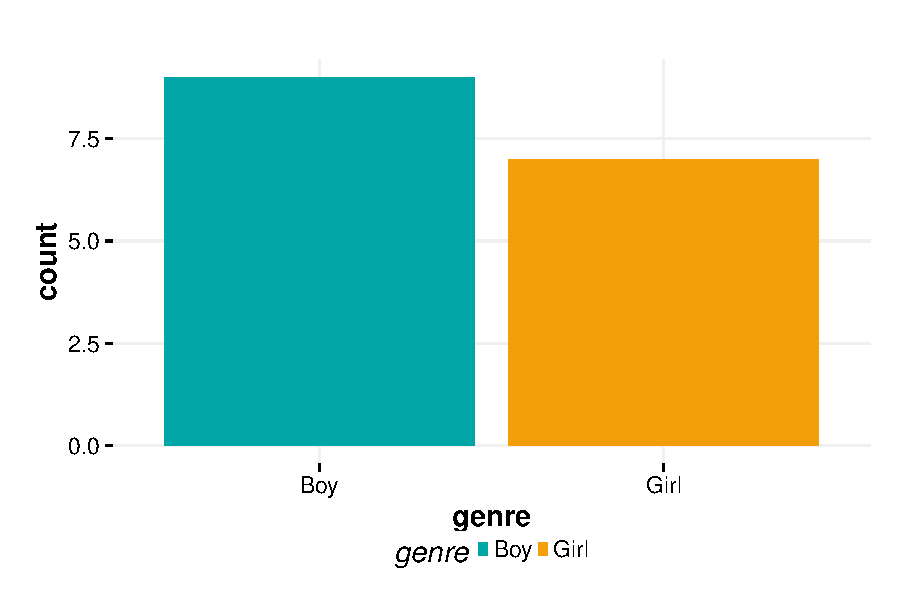
\includegraphics{interviews-plot_gender}

\subsubsection{Age}
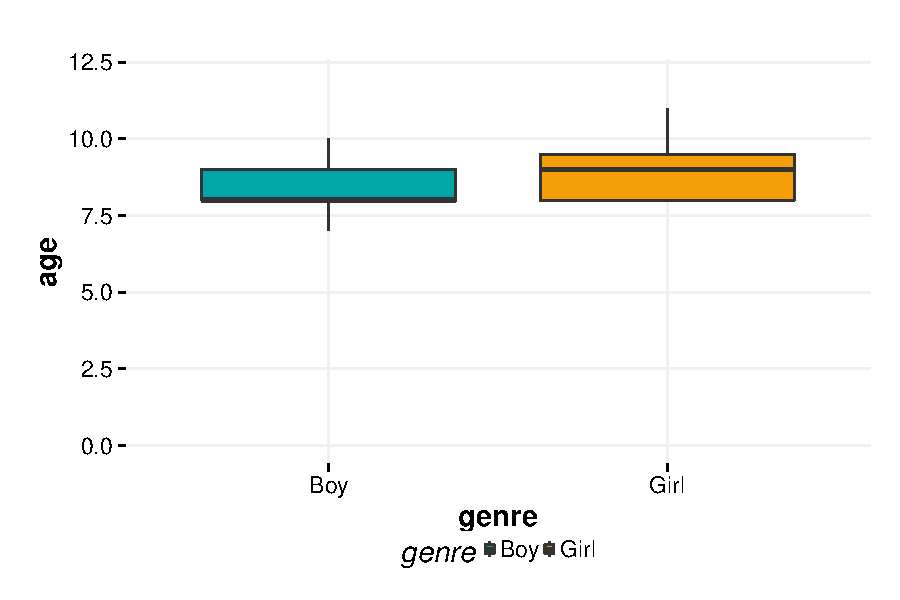
\includegraphics{interviews-plot_gender_age}

\subsubsection{order}
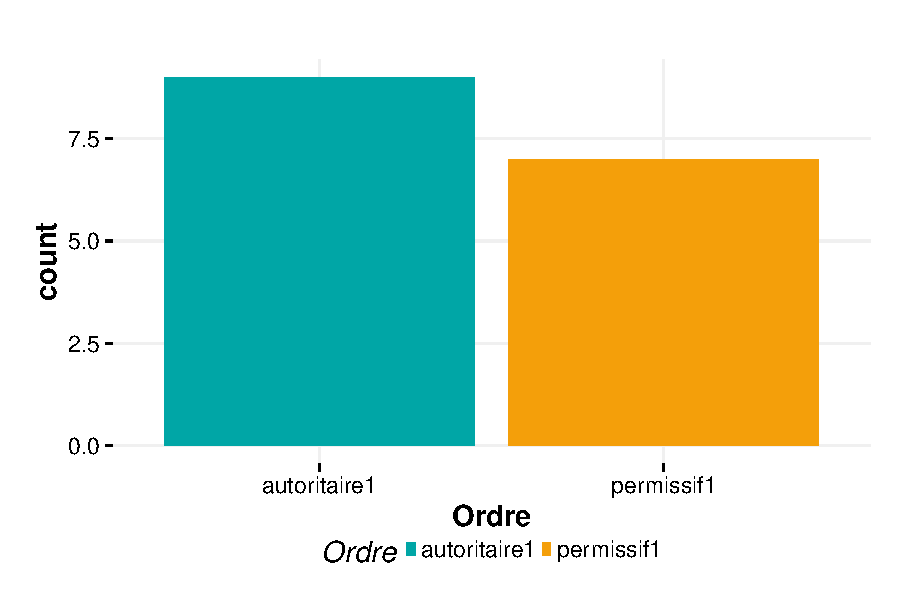
\includegraphics{interviews-plot_order}

\subsubsection{Preferred style parent}
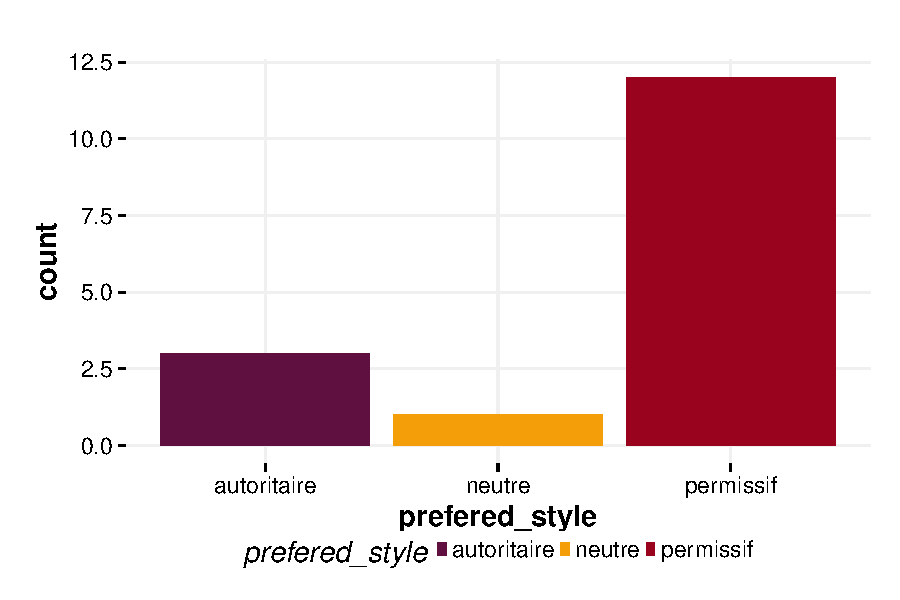
\includegraphics{interviews-plot_preferred_style_parent}

\subsubsection{Preferred style children}
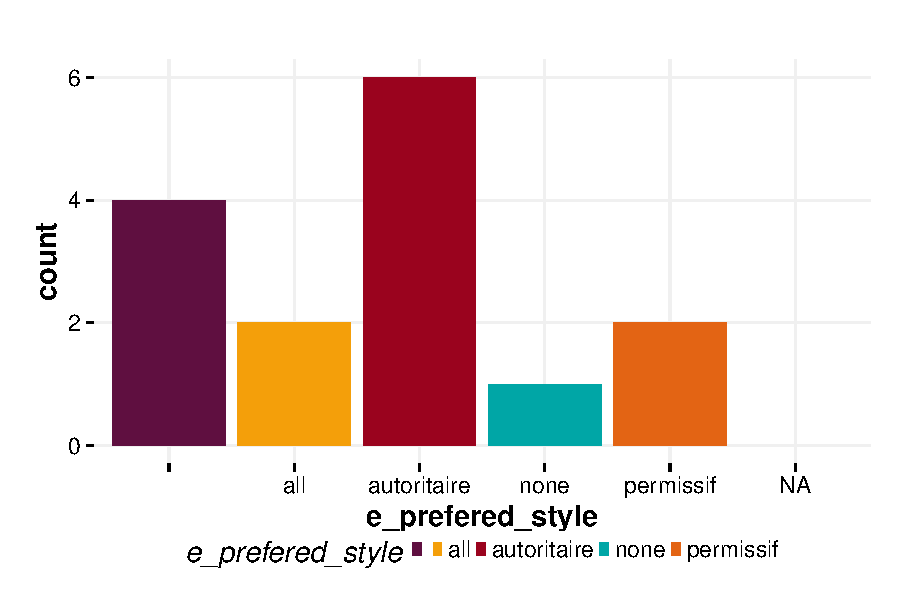
\includegraphics{interviews-plot_preferred_style_child}

\subsection{COIRS - CHILD ORIENTAION IN INTERACTING WITH ROBOT}

The following plot shows the average ranking for children for each of the object (1: first in the child's wish list)

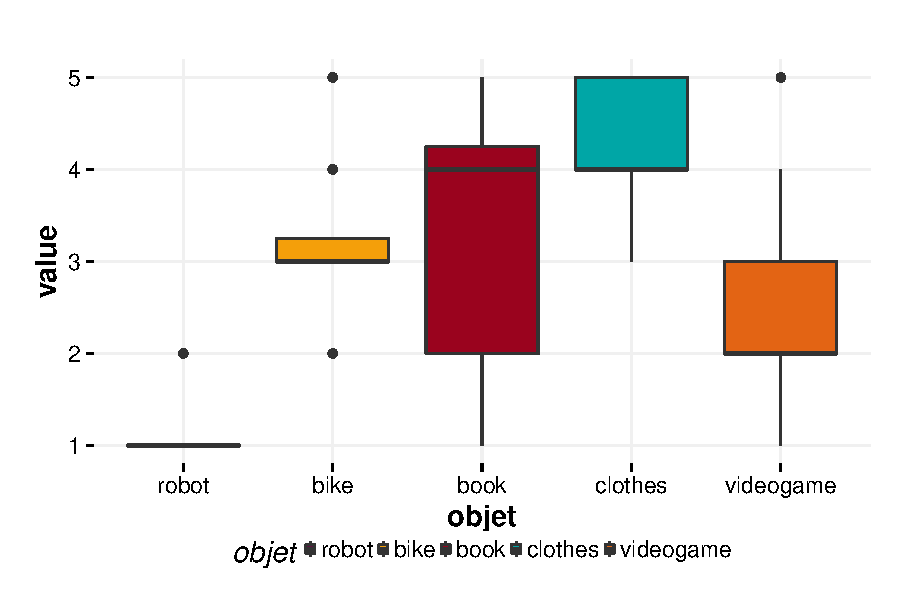
\includegraphics{interviews-plot_coirs_child}

The following plot shows the average ranking for parents for each of the object (1: first in the parent's wish list as a gift for thei child)
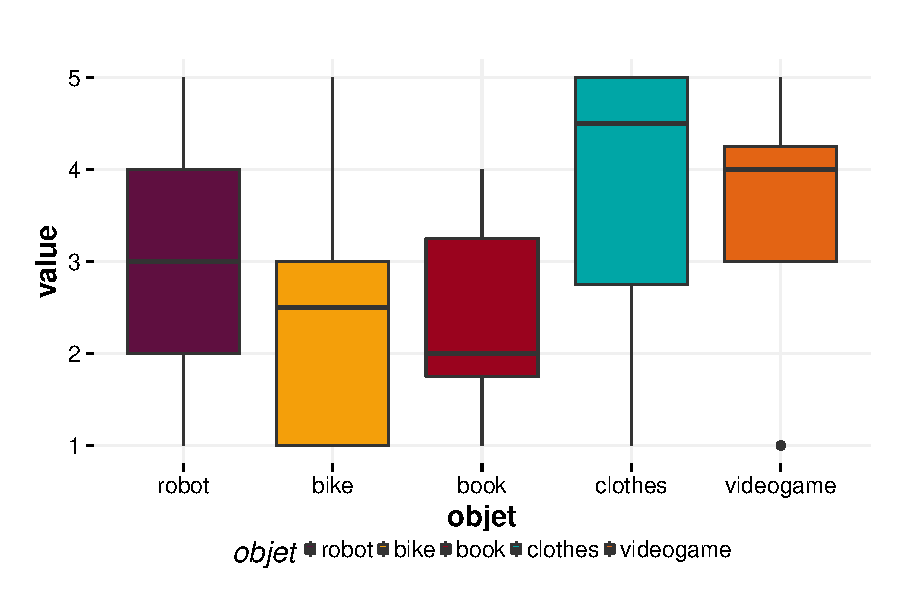
\includegraphics{interviews-plot_coirs_parent}

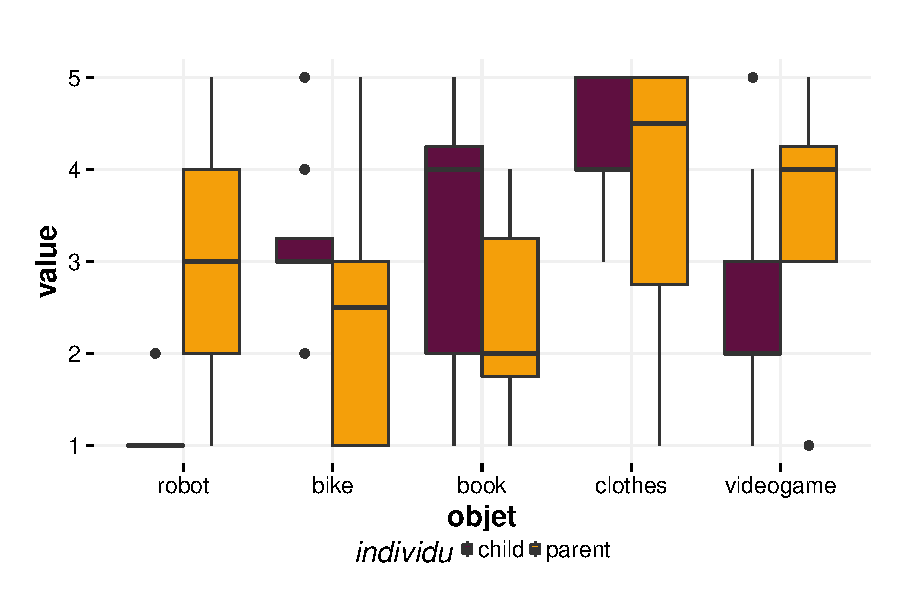
\includegraphics{interviews-plot_coirs_parent_enfant}

\subsubsection{Child-parent correlation in object ranking} 
Next graphs show the correlation between parent and children ranking for each of the child subject\newline
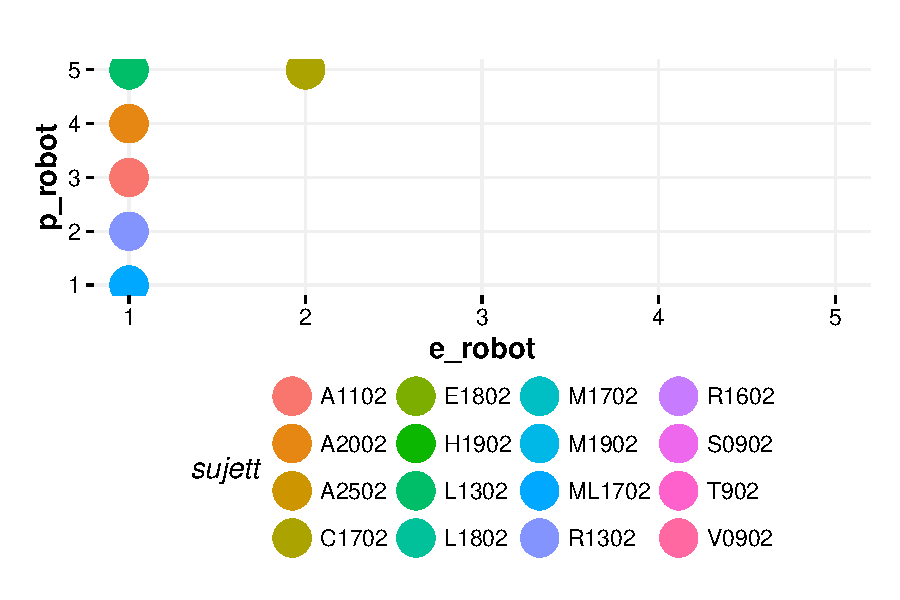
\includegraphics{interviews-plot_coirs_parent_enfant_robot}

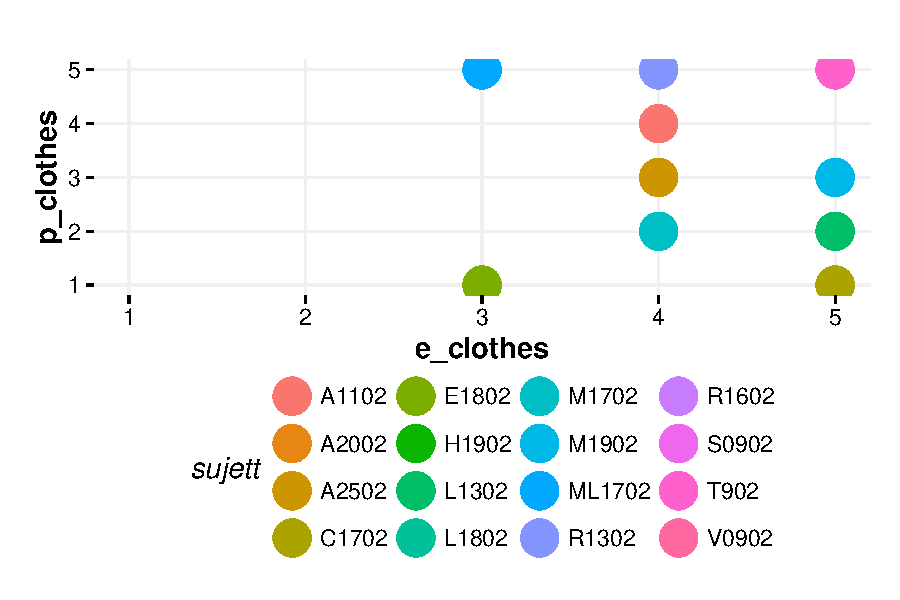
\includegraphics{interviews-plot_coirs_parent_enfant_clothes}

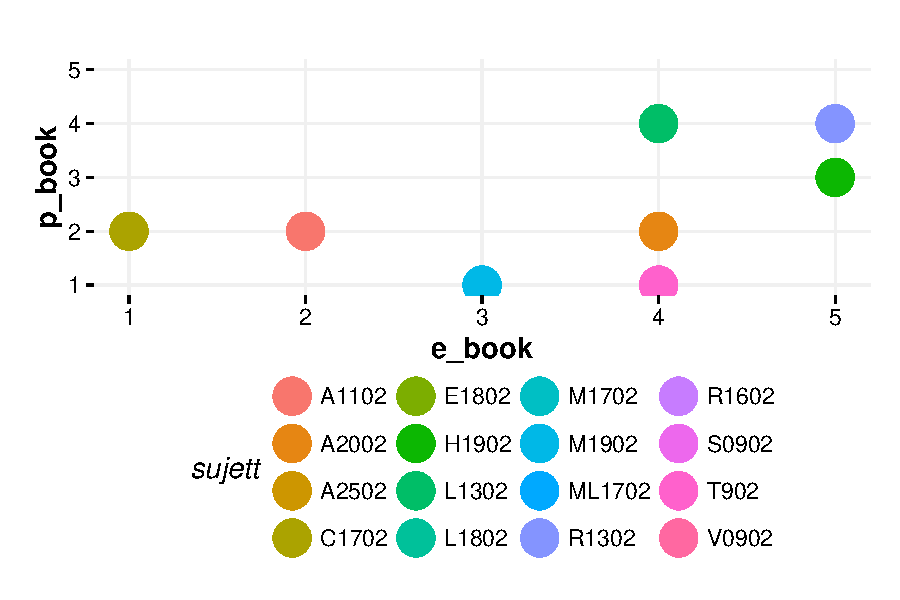
\includegraphics{interviews-plot_coirs_parent_enfant_book}

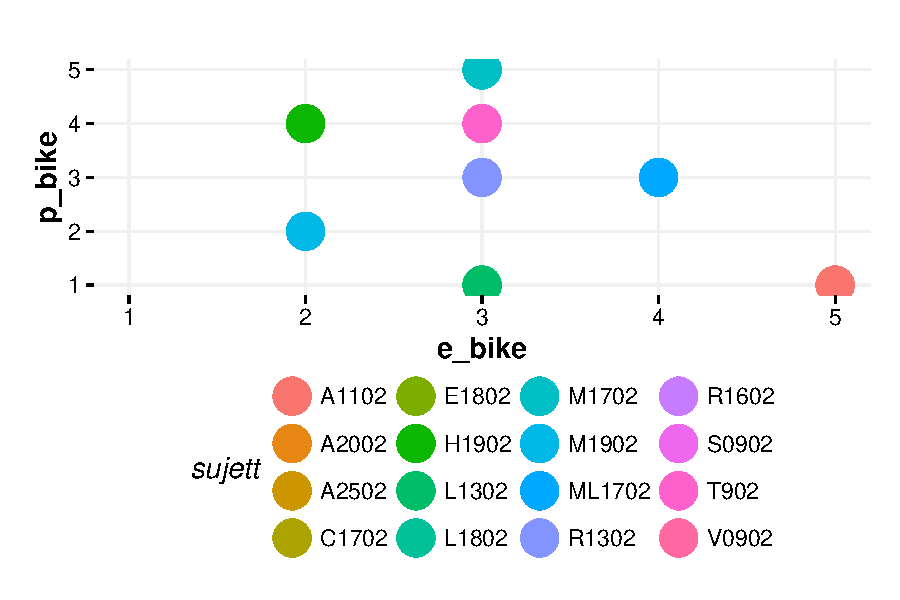
\includegraphics{interviews-plot_coirs_parent_enfant_bike}

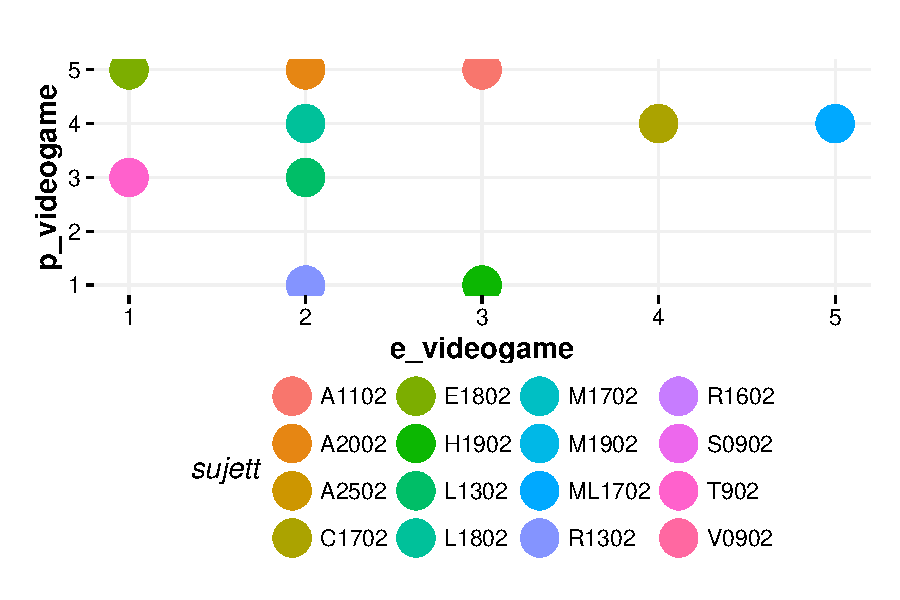
\includegraphics{interviews-plot_coirs_parent_enfant_videogame}

\subsection{Functionality preferences}

The following plot shows the average preference of children for each functionality (4: very preferred, 1: not preferred)
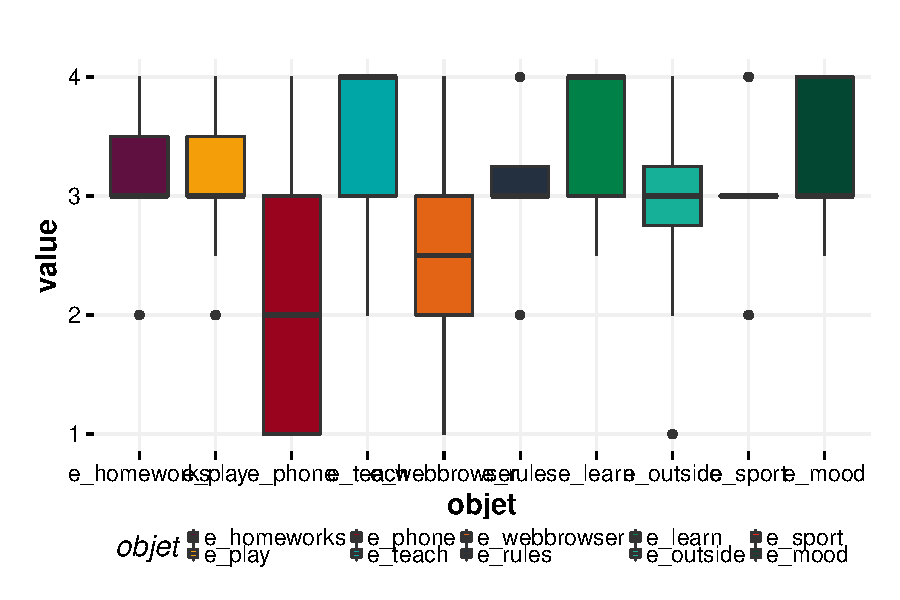
\includegraphics{interviews-plot_functionality_child}

The following plot shows the average preference of parents for each functionality (4: very preferred, 1: not preferred)
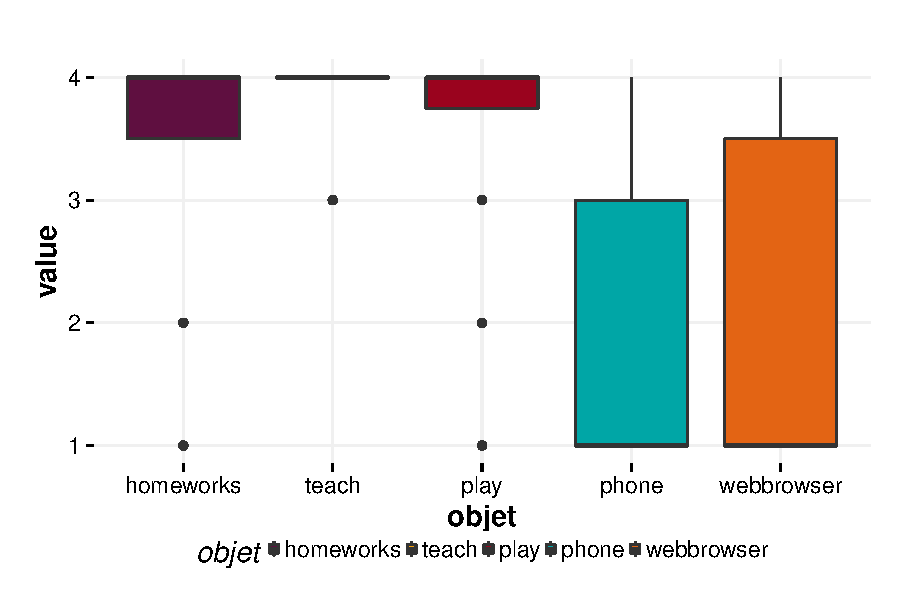
\includegraphics{interviews-plot_functionality_parent}

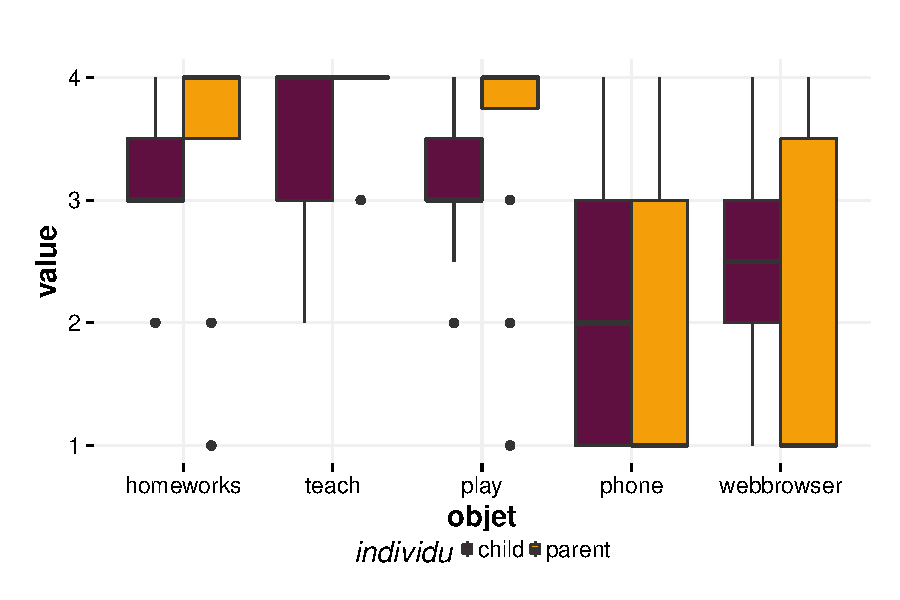
\includegraphics{interviews-plot_functionality_parent_enfant}


\begin{Schunk}
\begin{Soutput}
        objet individu  N    value        sd        se        ci
1   homeworks    child 13 3.115385 0.6504436 0.1804006 0.3930592
2   homeworks   parent 16 3.375000 1.1474610 0.2868652 0.6114388
3       teach    child 12 3.500000 0.6741999 0.1946247 0.4283662
4       teach   parent 16 3.937500 0.2500000 0.0625000 0.1332156
5        play    child 13 3.115385 0.6175842 0.1712870 0.3732024
6        play   parent 16 3.562500 0.8920949 0.2230237 0.4753638
7       phone    child 13 2.307692 1.1094004 0.3076923 0.6704039
8       phone   parent 15 1.866667 1.3020131 0.3361783 0.7210308
9  webbrowser    child 13 2.500000 0.9574271 0.2655425 0.5785674
10 webbrowser   parent 15 2.066667 1.3345233 0.3445724 0.7390344
\end{Soutput}
\end{Schunk}
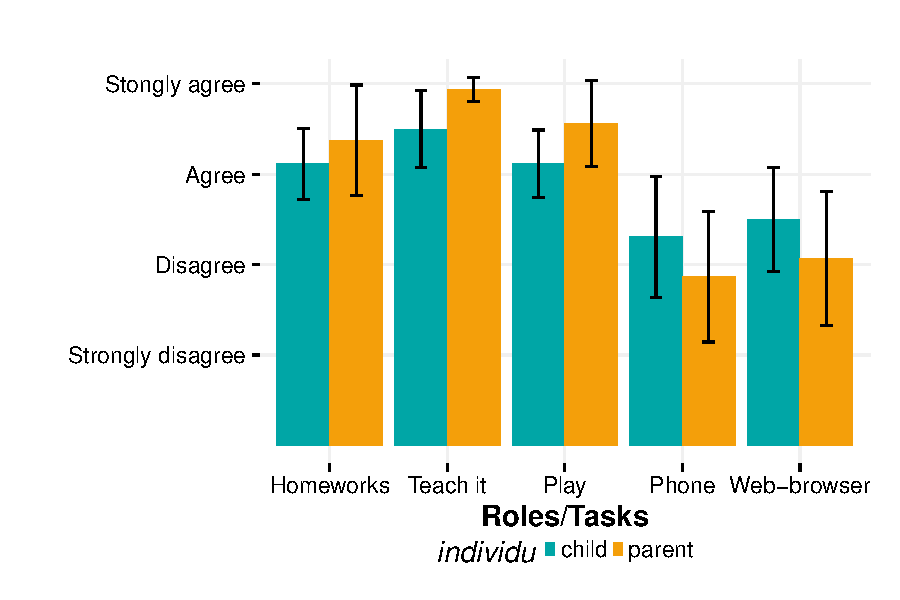
\includegraphics{interviews-plot_functionality_parent_enfant_bar}
\begin{Schunk}
\begin{Sinput}
> attach(df)
> summary(df)
\end{Sinput}
\begin{Soutput}
     sujett         age          genre             Ordre      individu        
 A1102  : 10   Min.   : 7.000   Boy :90   autoritaire1:90   Length:160        
 A2002  : 10   1st Qu.: 8.000   Girl:70   permissif1  :70   Class :character  
 A2502  : 10   Median : 8.500                               Mode  :character  
 C1702  : 10   Mean   : 8.688                                                 
 E1802  : 10   3rd Qu.: 9.000                                                 
 H1902  : 10   Max.   :11.000                                                 
 (Other):100                                                                  
        objet        value      
 homeworks :32   Min.   :1.000  
 teach     :32   1st Qu.:2.000  
 play      :32   Median :3.000  
 phone     :32   Mean   :2.947  
 webbrowser:32   3rd Qu.:4.000  
                 Max.   :4.000  
                 NA's   :18     
\end{Soutput}
\begin{Sinput}
> summary(aov(df$value~df$objet*df$individu))
\end{Sinput}
\begin{Soutput}
                      Df Sum Sq Mean Sq F value   Pr(>F)    
df$objet               4  60.25  15.062  16.335 6.81e-11 ***
df$individu            1   0.11   0.112   0.121    0.729    
df$objet:df$individu   4   5.78   1.445   1.567    0.187    
Residuals            132 121.71   0.922                     
---
Signif. codes:  0 ‘***’ 0.001 ‘**’ 0.01 ‘*’ 0.05 ‘.’ 0.1 ‘ ’ 1
18 observations deleted due to missingness
\end{Soutput}
\end{Schunk}

\subsubsection{Child-parent correlation in functionality preferrence} 
Next graphs show the correlation between parent and children ranking for each of the child subject\newline
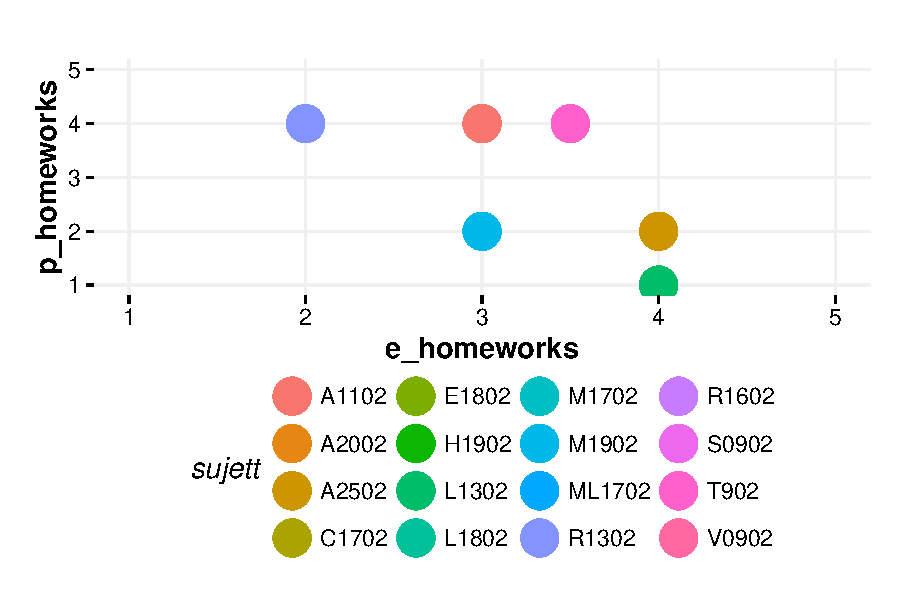
\includegraphics{interviews-plot_coirs_parent_enfant_hmk}

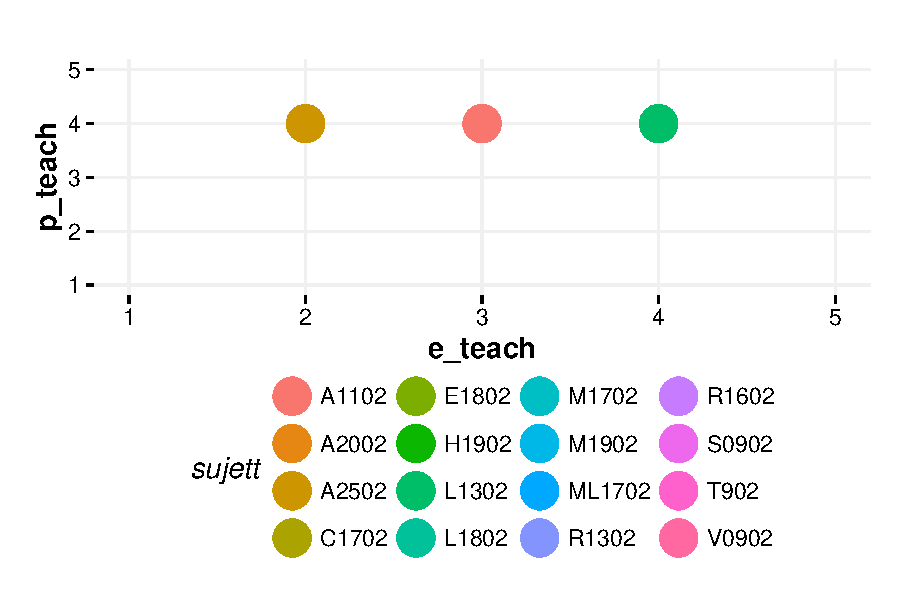
\includegraphics{interviews-plot_coirs_parent_enfant_teach}

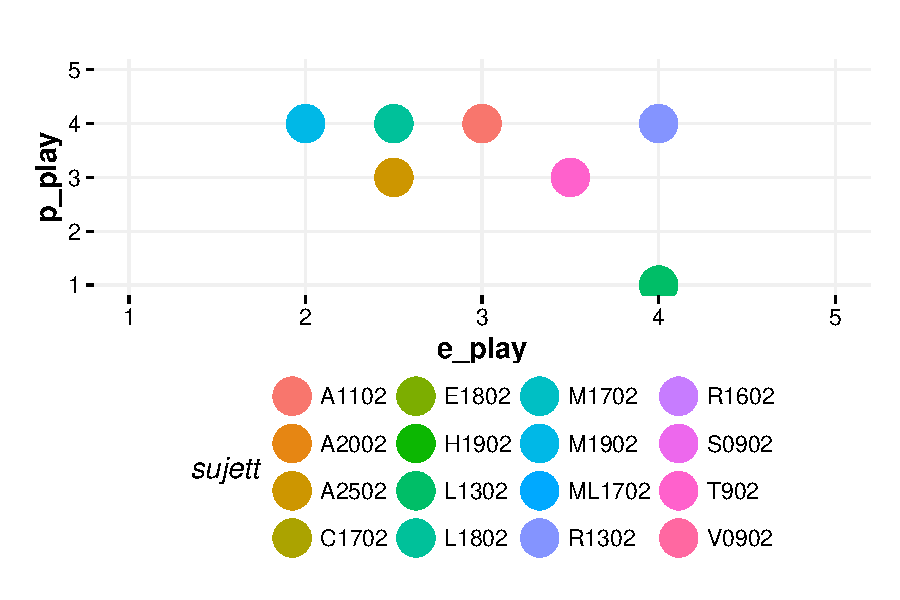
\includegraphics{interviews-plot_coirs_parent_enfant_play}

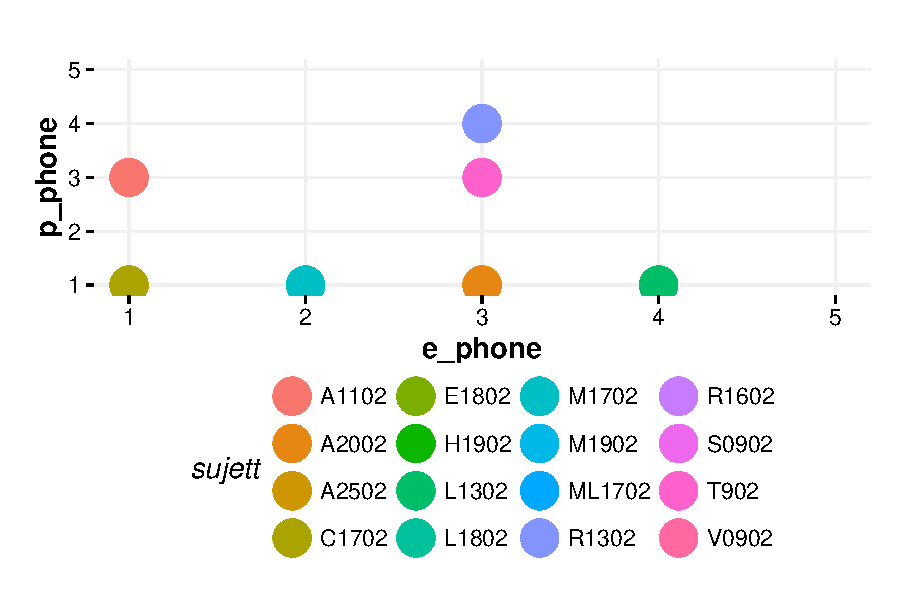
\includegraphics{interviews-plot_coirs_parent_enfant_phone}

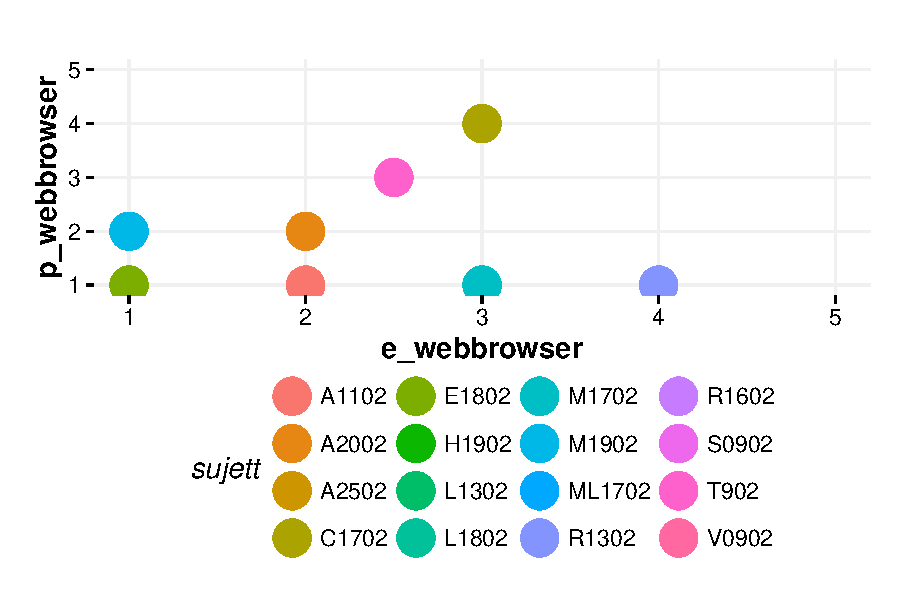
\includegraphics{interviews-plot_coirs_parent_enfant_webbrowser}



\section{Features}



\subsection{Static Features}
\subsubsection{Body Volume}
We filtered the data as follow


\textbf{Child}
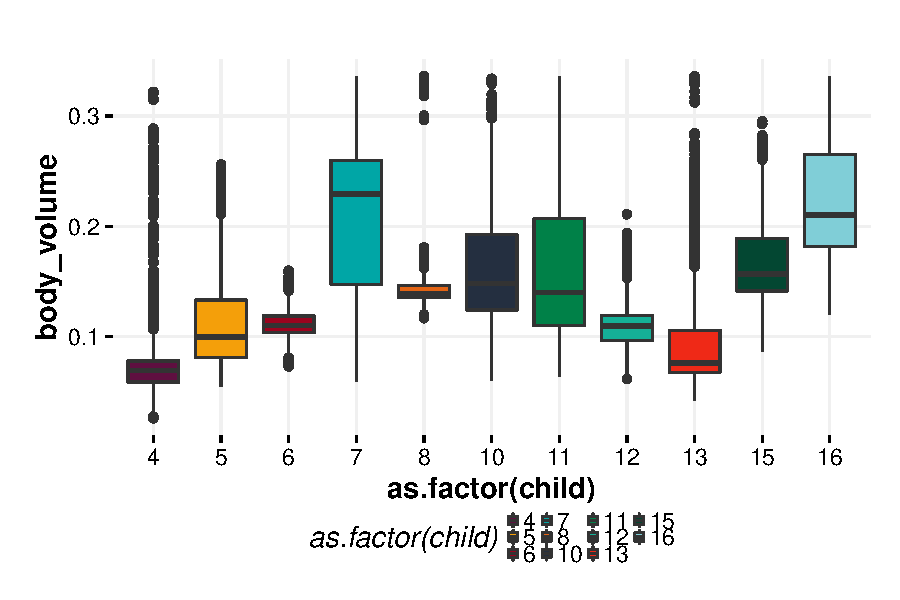
\includegraphics{features-plot_body_volume_child_quiz}

\begin{Schunk}
\begin{Soutput}
Error: session
              Df Sum Sq Mean Sq
factor(child)  1  49.97   49.97

Error: style
              Df Sum Sq Mean Sq
factor(child)  1 0.5028  0.5028

Error: session:style
              Df Sum Sq Mean Sq
factor(child)  1  91.12   91.12

Error: Within
                  Df Sum Sq Mean Sq F value Pr(>F)    
factor(child)      9  152.5  16.941    7978 <2e-16 ***
Residuals     138529  294.2   0.002                   
---
Signif. codes:  0 ‘***’ 0.001 ‘**’ 0.01 ‘*’ 0.05 ‘.’ 0.1 ‘ ’ 1
\end{Soutput}
\end{Schunk}

\textbf{Age}
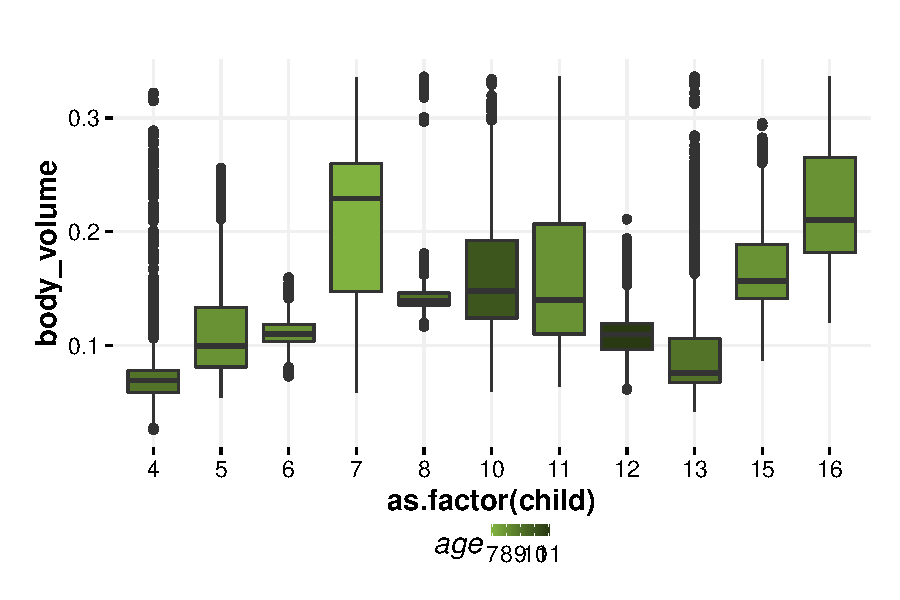
\includegraphics{features-plot_body_volume_child_age_quiz}

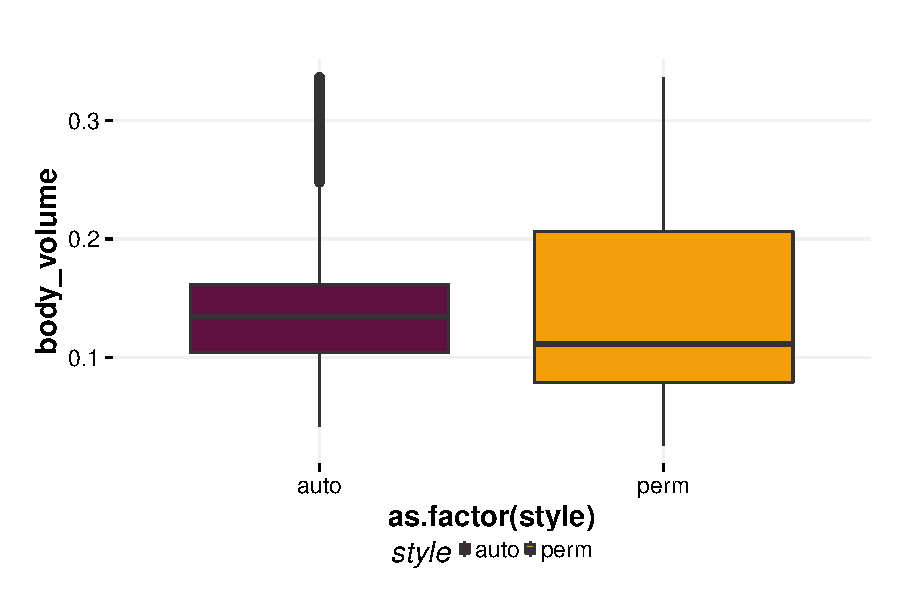
\includegraphics{features-plot_body_volume_style_quiz}

\begin{Schunk}
\begin{Soutput}
                Df Sum Sq Mean Sq F value Pr(>F)    
factor(age)      4  185.0   46.24   15883 <2e-16 ***
Residuals   138537  403.3    0.00                   
---
Signif. codes:  0 ‘***’ 0.001 ‘**’ 0.01 ‘*’ 0.05 ‘.’ 0.1 ‘ ’ 1
15181 observations deleted due to missingness
\end{Soutput}
\end{Schunk}

\textbf{Gender}
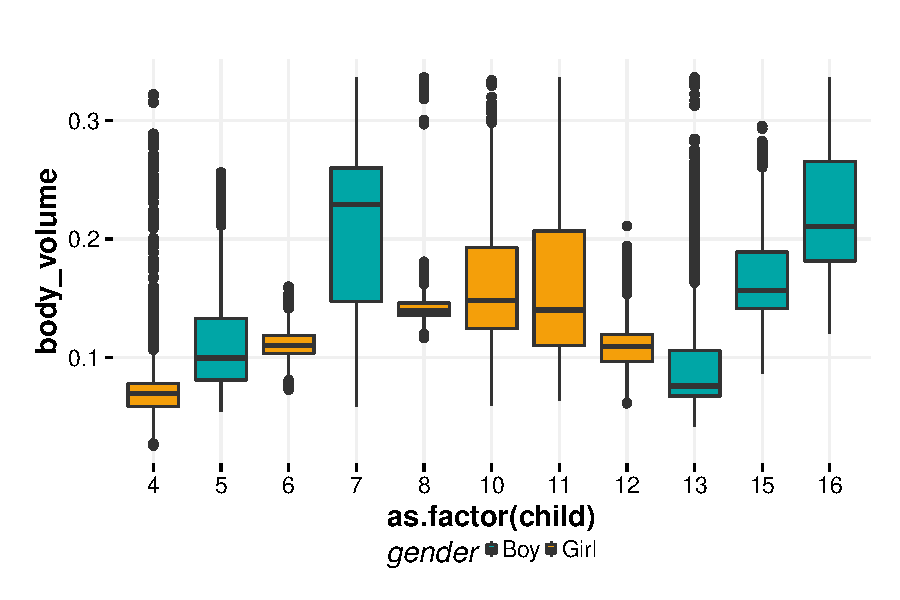
\includegraphics{features-plot_body_volume_child_gender_quiz}

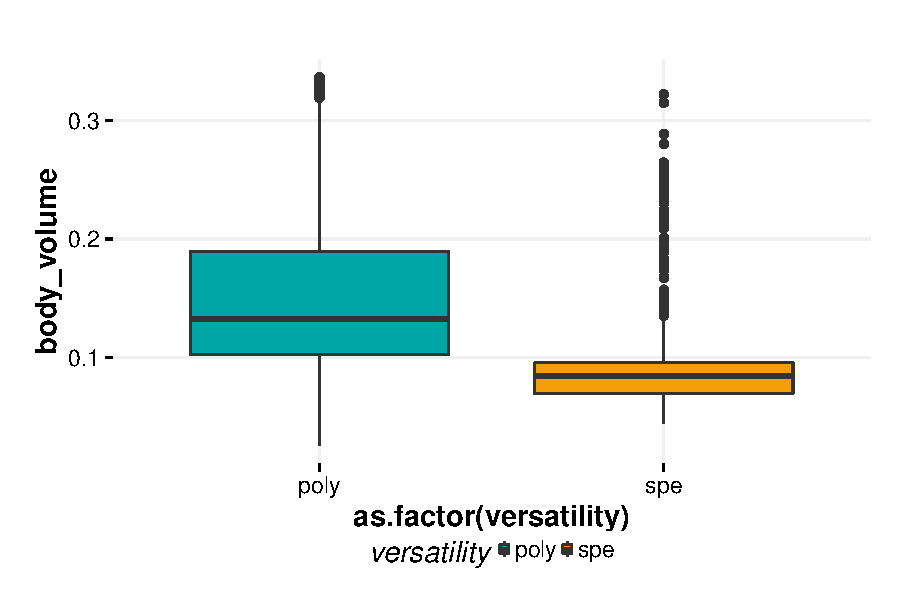
\includegraphics{features-plot_body_volume_gender_quiz}

\begin{Schunk}
\begin{Soutput}
                   Df Sum Sq Mean Sq F value Pr(>F)    
factor(gender)      1   22.5  22.472    5503 <2e-16 ***
Residuals      138540  565.8   0.004                   
---
Signif. codes:  0 ‘***’ 0.001 ‘**’ 0.01 ‘*’ 0.05 ‘.’ 0.1 ‘ ’ 1
15181 observations deleted due to missingness
\end{Soutput}
\end{Schunk}


\textbf{Versatility}
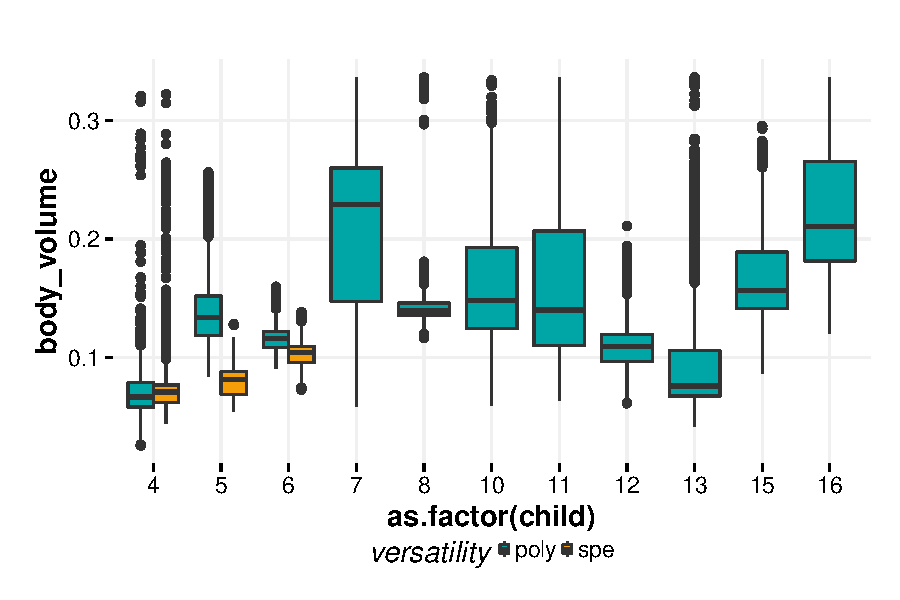
\includegraphics{features-plot_body_volume_child_versatility_quiz}

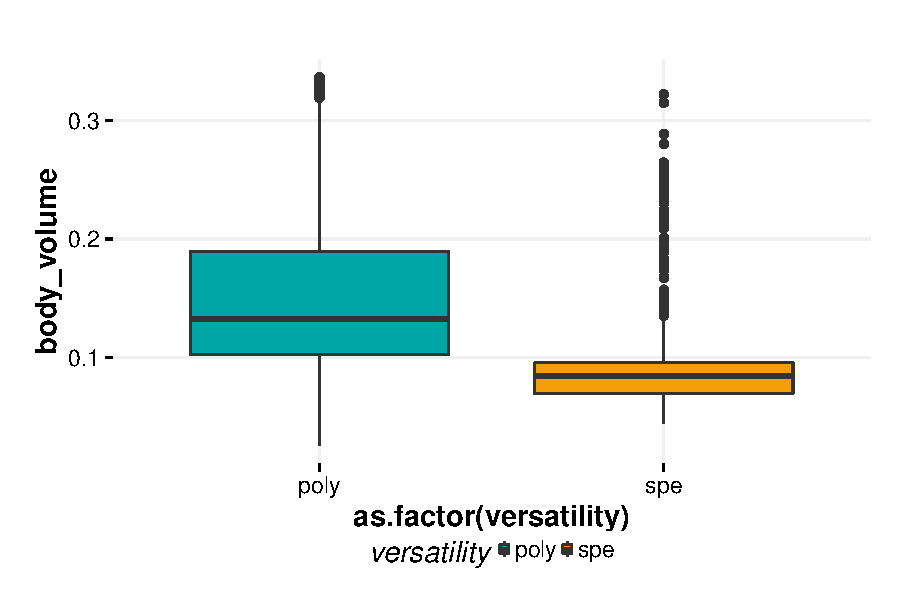
\includegraphics{features-plot_body_volume_gender_quiz}

\begin{Schunk}
\begin{Soutput}
                        Df Sum Sq Mean Sq F value Pr(>F)    
factor(versatility)      1   56.2   56.19   14631 <2e-16 ***
Residuals           138540  532.1    0.00                   
---
Signif. codes:  0 ‘***’ 0.001 ‘**’ 0.01 ‘*’ 0.05 ‘.’ 0.1 ‘ ’ 1
15181 observations deleted due to missingness
\end{Soutput}
\end{Schunk}


\textbf{Session}
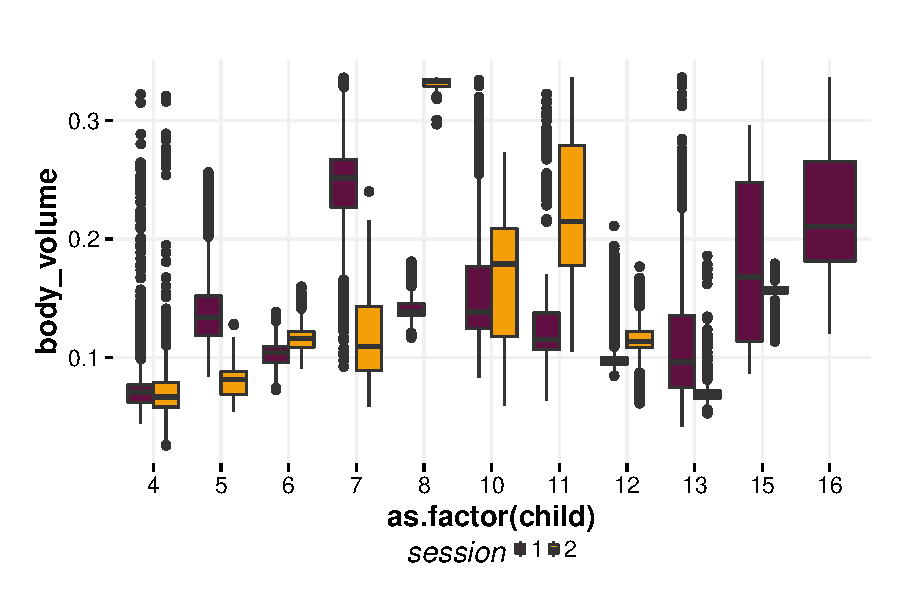
\includegraphics{features-plot_body_volume_child_session_quiz}

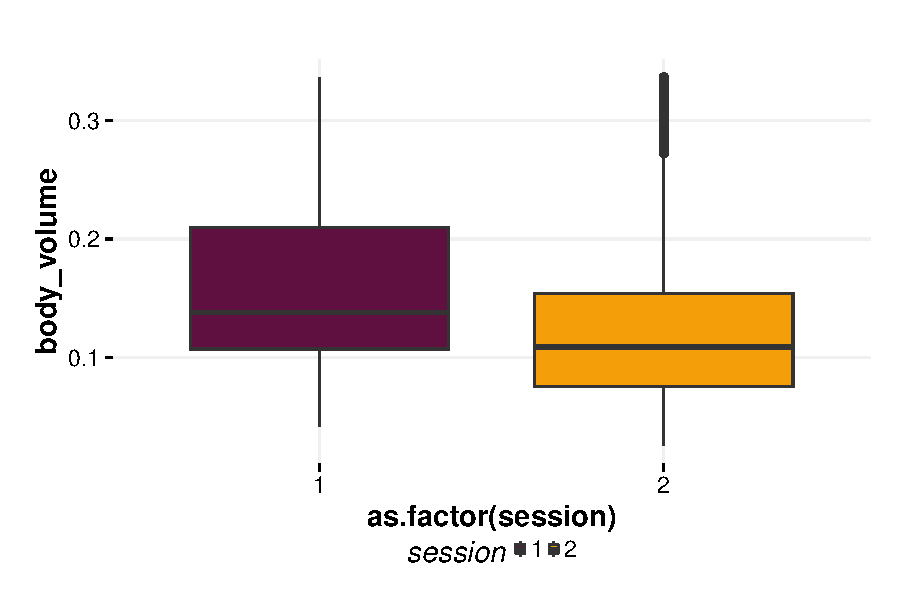
\includegraphics{features-plot_body_volume_session_quiz}

\begin{Schunk}
\begin{Soutput}
Error: child
                Df Sum Sq Mean Sq F value Pr(>F)  
factor(session)  1  124.1   124.1   7.131 0.0256 *
Residuals        9  156.6    17.4                 
---
Signif. codes:  0 ‘***’ 0.001 ‘**’ 0.01 ‘*’ 0.05 ‘.’ 0.1 ‘ ’ 1

Error: Within
                    Df Sum Sq Mean Sq F value Pr(>F)    
factor(session)      1  13.29  13.287    6256 <2e-16 ***
Residuals       138530 294.22   0.002                   
---
Signif. codes:  0 ‘***’ 0.001 ‘**’ 0.01 ‘*’ 0.05 ‘.’ 0.1 ‘ ’ 1
\end{Soutput}
\end{Schunk}

\textbf{Style}
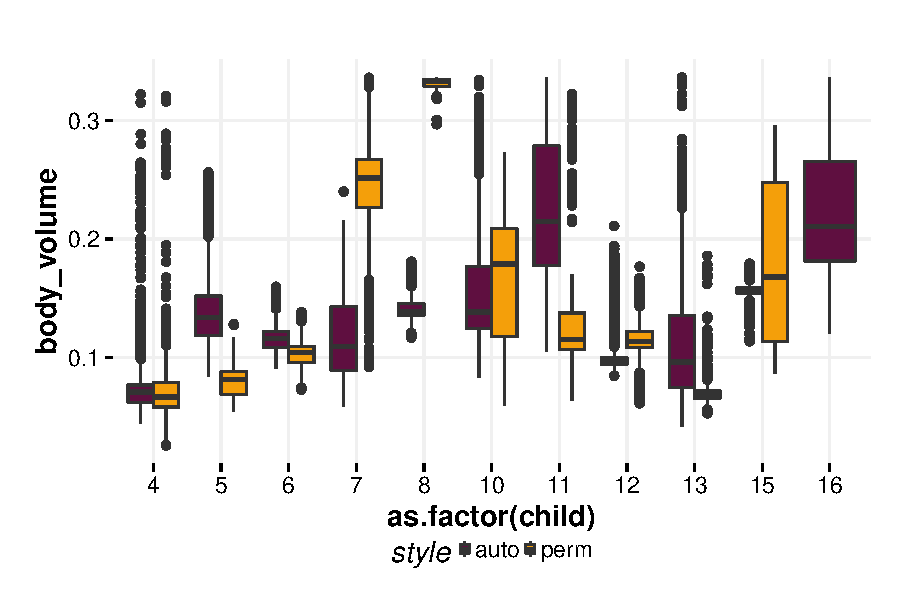
\includegraphics{features-plot_body_volume_child_style_quiz}

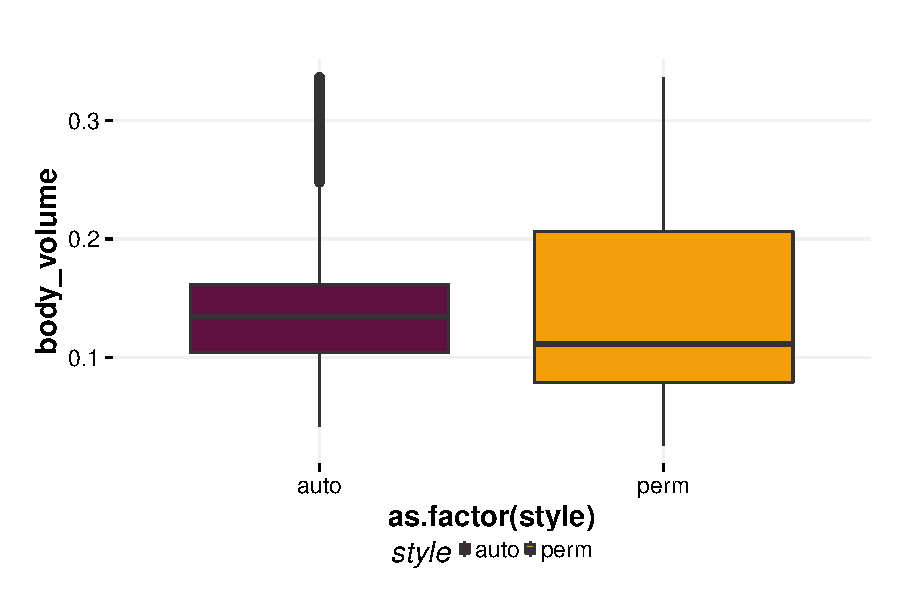
\includegraphics{features-plot_body_volume_style_quiz}

\begin{Schunk}
\begin{Soutput}
Error: child
              Df Sum Sq Mean Sq F value Pr(>F)
factor(style)  1   0.47   0.473   0.015  0.905
Residuals      9 280.26  31.140               

Error: Within
                  Df Sum Sq Mean Sq F value  Pr(>F)   
factor(style)      1   0.02 0.02324   10.47 0.00121 **
Residuals     138530 307.48 0.00222                   
---
Signif. codes:  0 ‘***’ 0.001 ‘**’ 0.01 ‘*’ 0.05 ‘.’ 0.1 ‘ ’ 1
\end{Soutput}
\end{Schunk}

\subsubsection{Distance}
\textbf{Child}
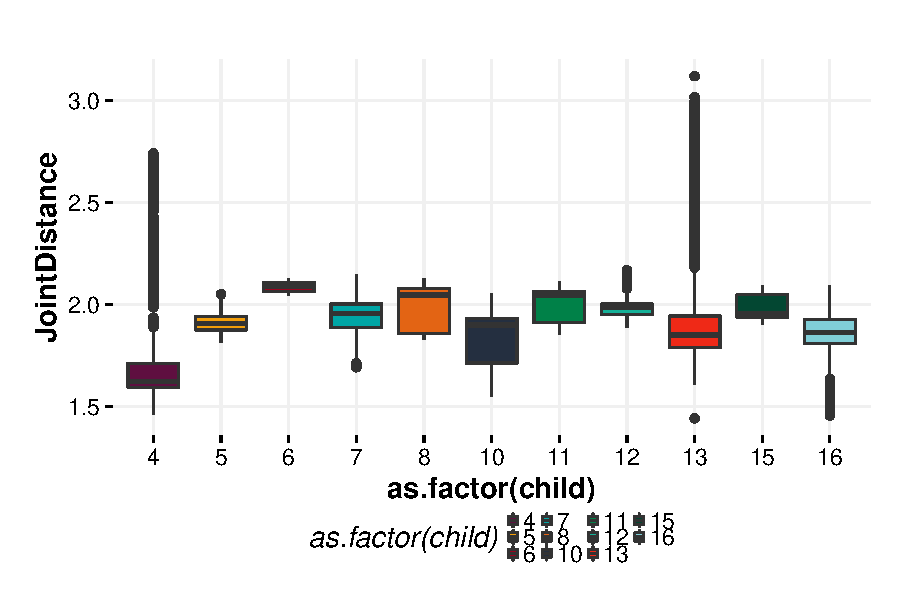
\includegraphics{features-plot_distance_child_quiz}

\begin{Schunk}
\begin{Soutput}
Error: session
              Df Sum Sq Mean Sq
factor(child)  1  60.39   60.39

Error: style
              Df Sum Sq Mean Sq
factor(child)  1  35.92   35.92

Error: session:style
              Df Sum Sq Mean Sq
factor(child)  1  626.8   626.8

Error: Within
                  Df Sum Sq Mean Sq F value Pr(>F)    
factor(child)      9  882.9   98.10    9457 <2e-16 ***
Residuals     153710 1594.5    0.01                   
---
Signif. codes:  0 ‘***’ 0.001 ‘**’ 0.01 ‘*’ 0.05 ‘.’ 0.1 ‘ ’ 1
\end{Soutput}
\end{Schunk}

\textbf{Age}
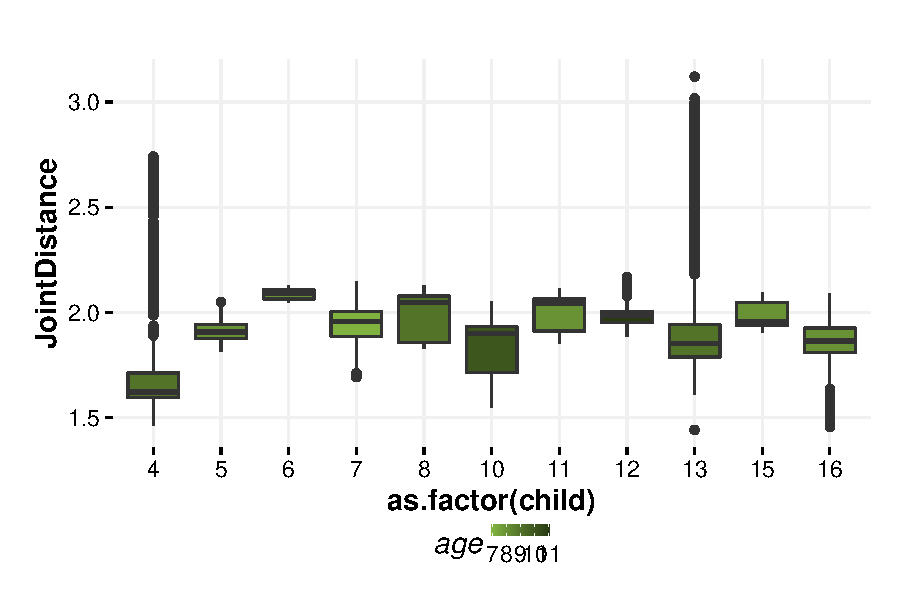
\includegraphics{features-plot_distance_child_age_quiz}

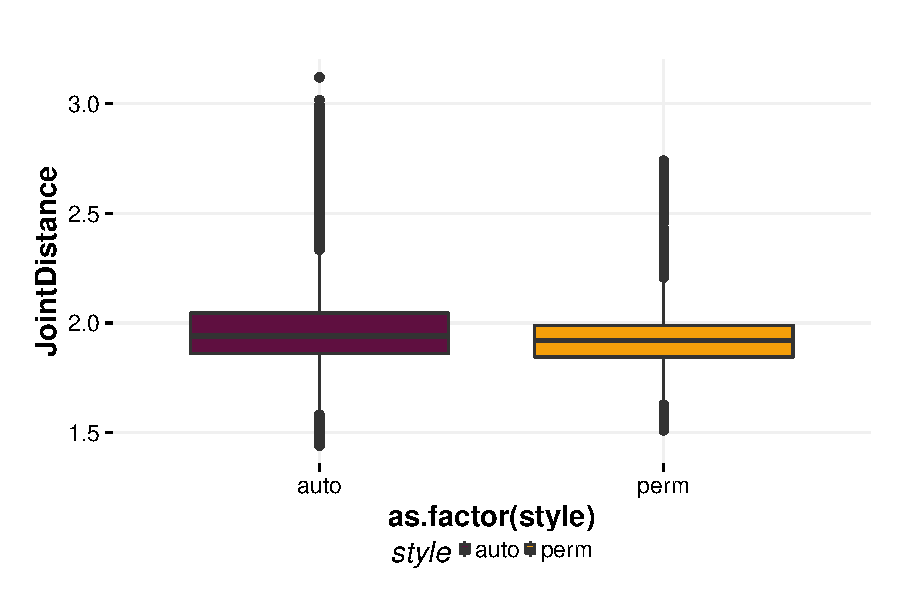
\includegraphics{features-plot_distance_style_quiz}

\begin{Schunk}
\begin{Soutput}
                Df Sum Sq Mean Sq F value Pr(>F)    
factor(age)      4  665.1  166.27   10080 <2e-16 ***
Residuals   153718 2535.4    0.02                   
---
Signif. codes:  0 ‘***’ 0.001 ‘**’ 0.01 ‘*’ 0.05 ‘.’ 0.1 ‘ ’ 1
\end{Soutput}
\end{Schunk}

\textbf{Gender}
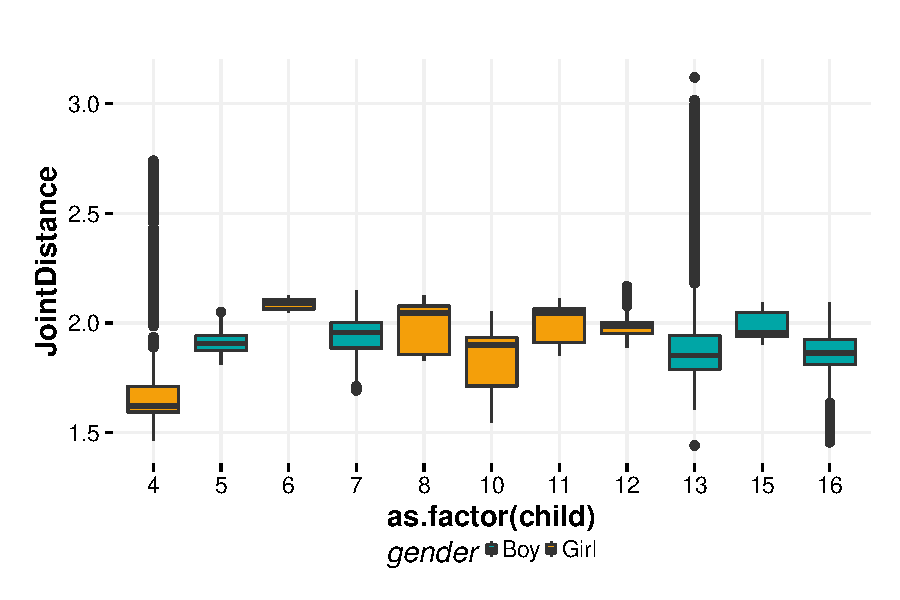
\includegraphics{features-plot_distance_child_gender_quiz}

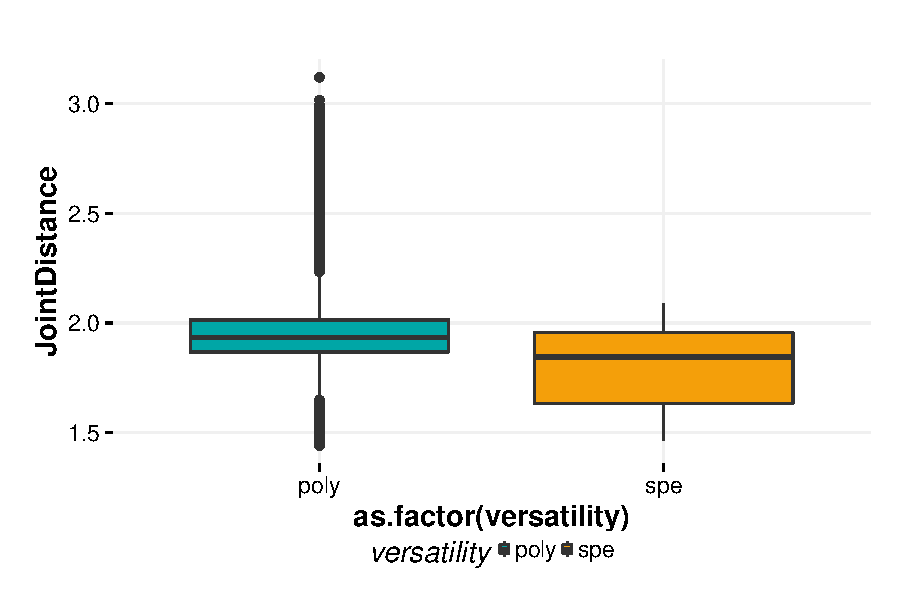
\includegraphics{features-plot_distance_gender_quiz}

\begin{Schunk}
\begin{Soutput}
                   Df Sum Sq Mean Sq F value Pr(>F)    
factor(gender)      1      5   5.478   263.6 <2e-16 ***
Residuals      153721   3195   0.021                   
---
Signif. codes:  0 ‘***’ 0.001 ‘**’ 0.01 ‘*’ 0.05 ‘.’ 0.1 ‘ ’ 1
\end{Soutput}
\end{Schunk}


\textbf{Versatility}
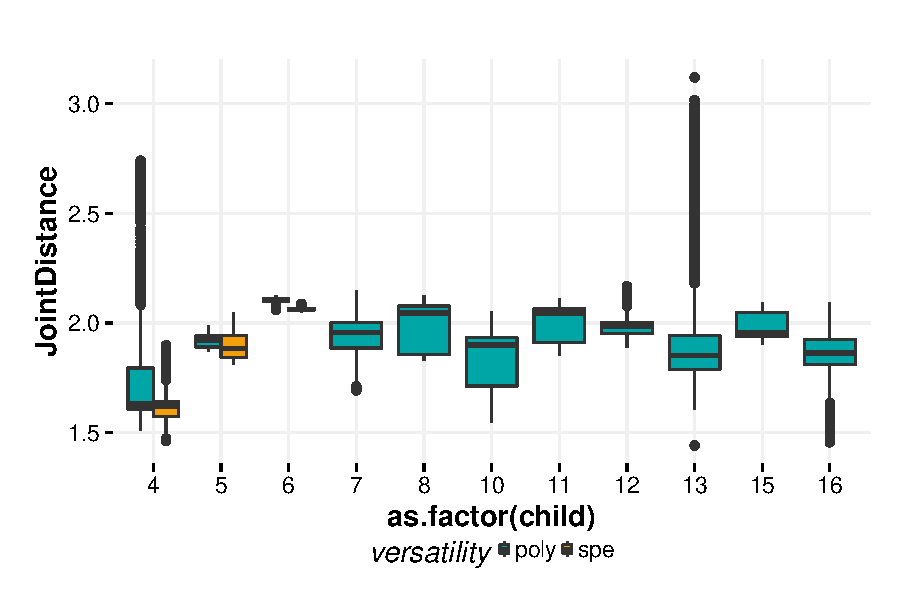
\includegraphics{features-plot_distance_child_versatility_quiz}

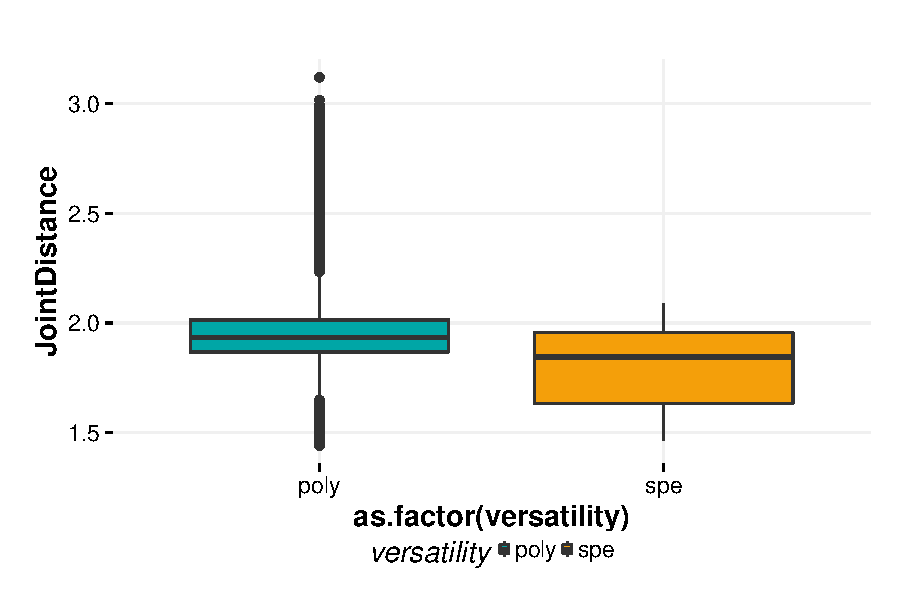
\includegraphics{features-plot_distance_gender_quiz}

\begin{Schunk}
\begin{Soutput}
                        Df Sum Sq Mean Sq F value Pr(>F)    
factor(versatility)      1  155.9  155.91    7872 <2e-16 ***
Residuals           153721 3044.6    0.02                   
---
Signif. codes:  0 ‘***’ 0.001 ‘**’ 0.01 ‘*’ 0.05 ‘.’ 0.1 ‘ ’ 1
\end{Soutput}
\end{Schunk}


\textbf{Session}
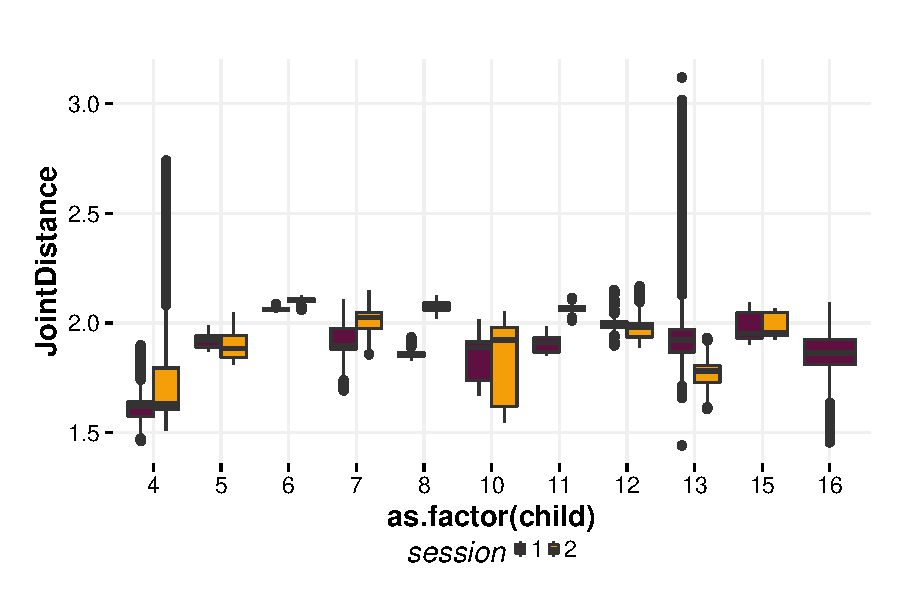
\includegraphics{features-plot_distance_child_session_quiz}

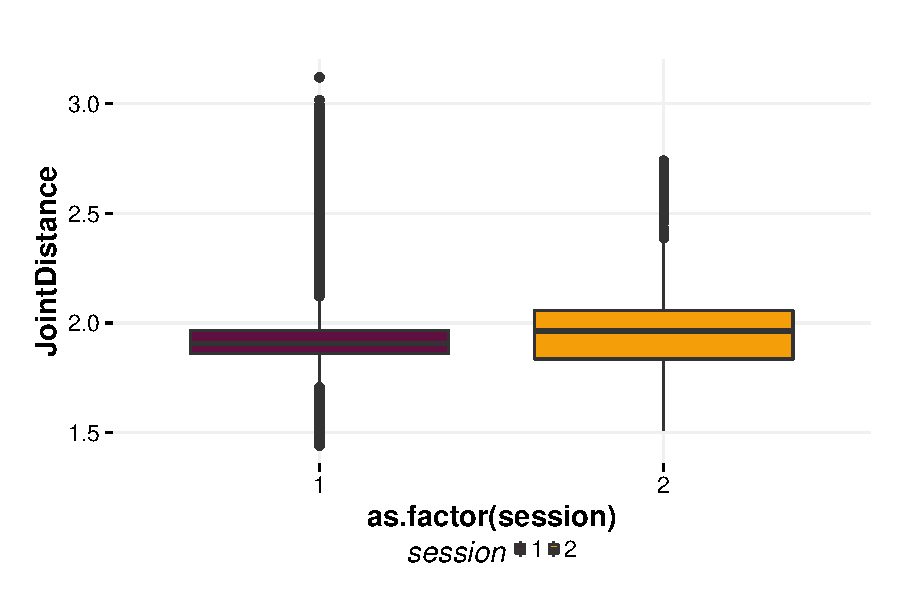
\includegraphics{features-plot_distance_session_quiz}

\begin{Schunk}
\begin{Soutput}
Error: child
                Df Sum Sq Mean Sq F value Pr(>F)
factor(session)  1   59.1   59.08   0.368  0.559
Residuals        9 1446.0  160.67               

Error: Within
                    Df Sum Sq Mean Sq F value Pr(>F)    
factor(session)      1   33.3   33.33    3082 <2e-16 ***
Residuals       153711 1662.1    0.01                   
---
Signif. codes:  0 ‘***’ 0.001 ‘**’ 0.01 ‘*’ 0.05 ‘.’ 0.1 ‘ ’ 1
\end{Soutput}
\end{Schunk}

\textbf{Style}
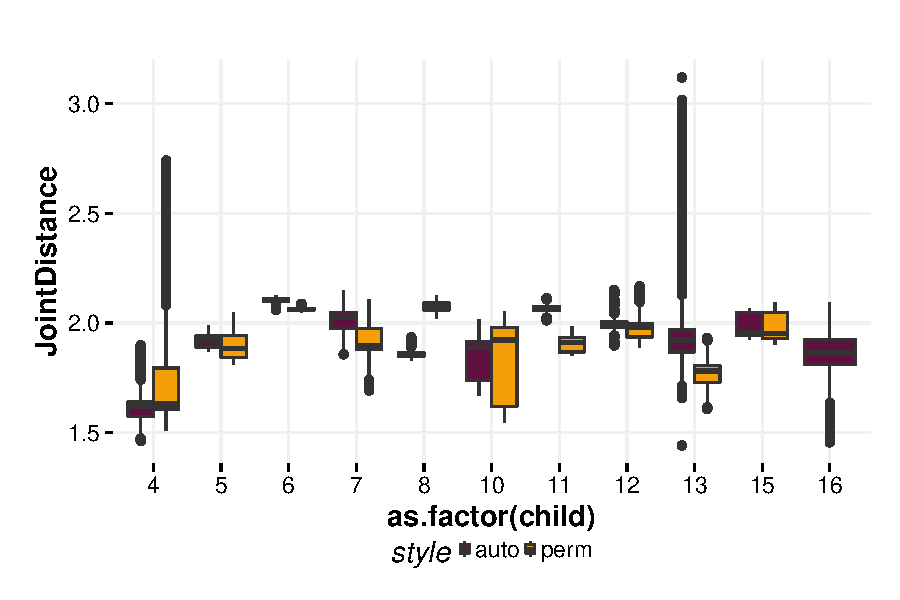
\includegraphics{features-plot_distance_child_style_quiz}

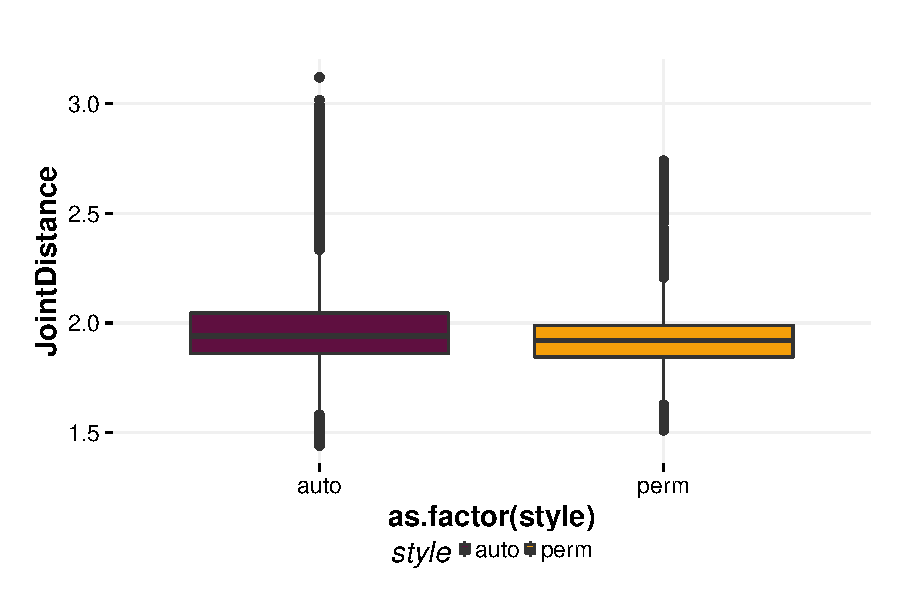
\includegraphics{features-plot_distance_style_quiz}

\begin{Schunk}
\begin{Soutput}
Error: child
              Df Sum Sq Mean Sq F value Pr(>F)
factor(style)  1   64.1   64.12     0.4  0.543
Residuals      9 1441.0  160.11               

Error: Within
                  Df Sum Sq Mean Sq F value Pr(>F)    
factor(style)      1   52.5   52.47    4909 <2e-16 ***
Residuals     153711 1642.9    0.01                   
---
Signif. codes:  0 ‘***’ 0.001 ‘**’ 0.01 ‘*’ 0.05 ‘.’ 0.1 ‘ ’ 1
\end{Soutput}
\end{Schunk}


\subsubsection{Center of Mass}

\subsubsection{Center of Mass Displacement}

\subsubsection{Distance Covered}

\subsubsection{Hand Relationship}

\subsubsection{Shoulder Angle}

\subsubsection{Elbow Flexion}

\subsubsection{Feet Relationship}

\subsubsection{Torso Neck Orientation}

\subsubsection{Body lean angle - Frontal}
\textbf{Child}
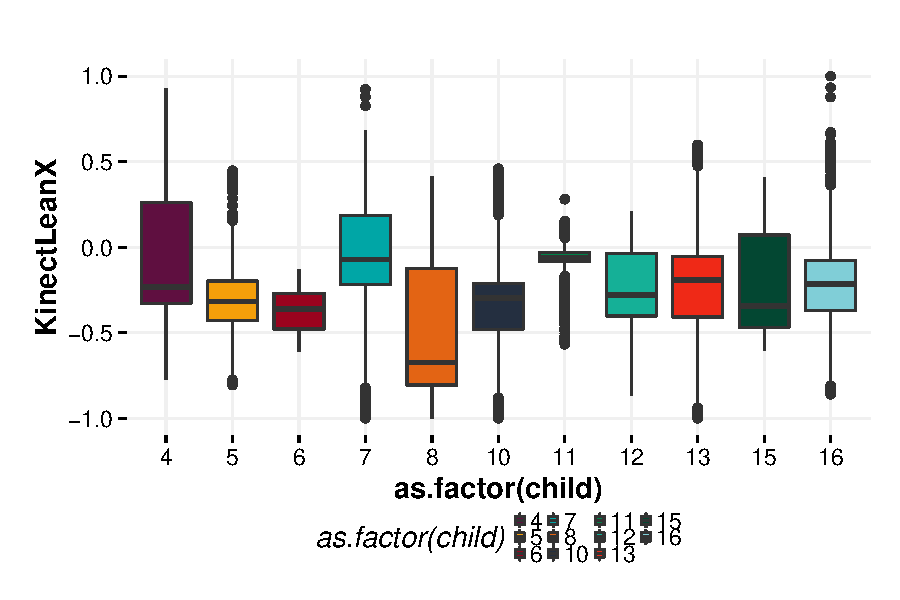
\includegraphics{features-plot_leanx_child_quiz}

\begin{Schunk}
\begin{Soutput}
Error: session
              Df Sum Sq Mean Sq
factor(child)  1   1307    1307

Error: style
              Df Sum Sq Mean Sq
factor(child)  1  6.239   6.239

Error: session:style
              Df Sum Sq Mean Sq
factor(child)  1  343.9   343.9

Error: Within
                  Df Sum Sq Mean Sq F value Pr(>F)    
factor(child)      9   1728  192.03    3762 <2e-16 ***
Residuals     153710   7845    0.05                   
---
Signif. codes:  0 ‘***’ 0.001 ‘**’ 0.01 ‘*’ 0.05 ‘.’ 0.1 ‘ ’ 1
\end{Soutput}
\end{Schunk}

\textbf{Age}
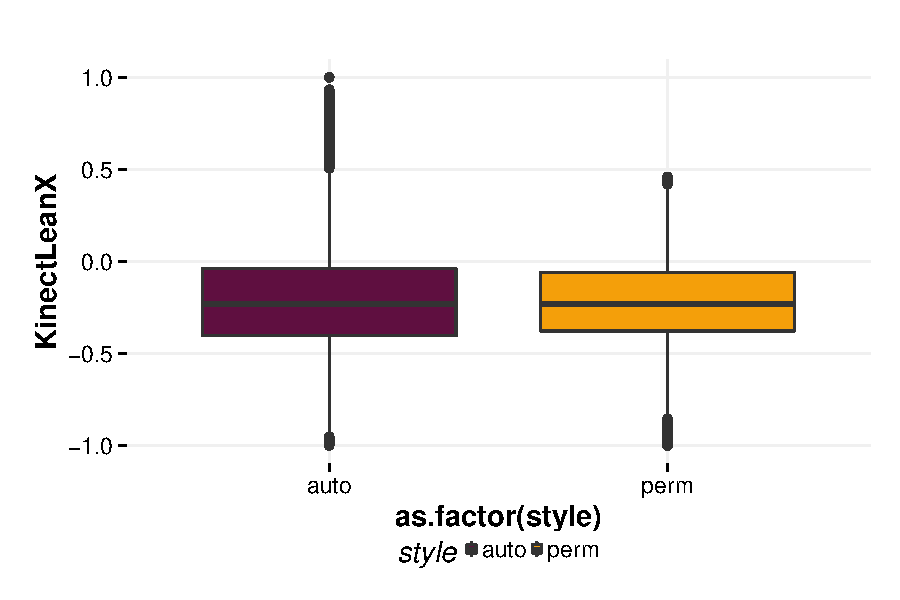
\includegraphics{features-plot_leanx_style_quiz}

\begin{Schunk}
\begin{Soutput}
                Df Sum Sq Mean Sq F value Pr(>F)    
factor(age)      4    743  185.85    2724 <2e-16 ***
Residuals   153718  10487    0.07                   
---
Signif. codes:  0 ‘***’ 0.001 ‘**’ 0.01 ‘*’ 0.05 ‘.’ 0.1 ‘ ’ 1
\end{Soutput}
\end{Schunk}

\textbf{Gender}
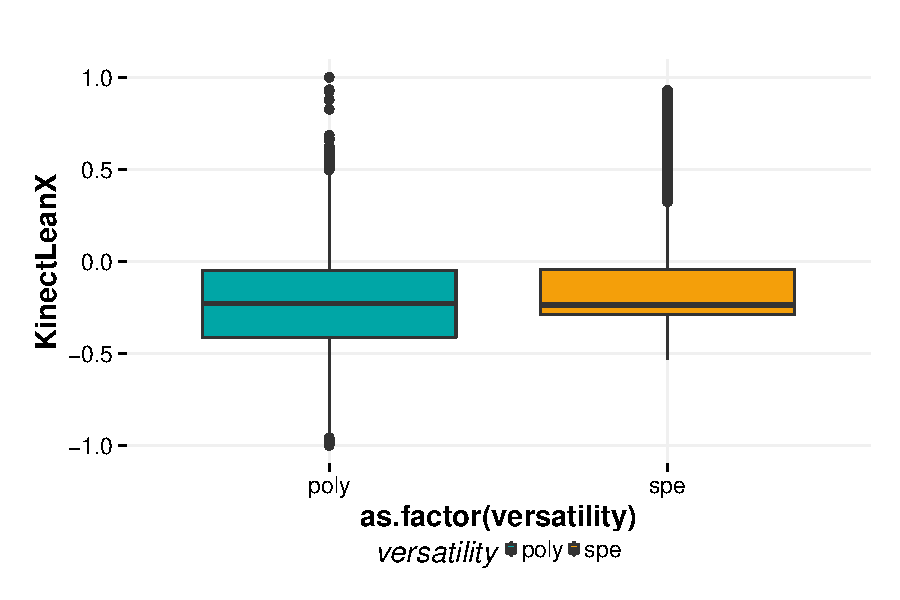
\includegraphics{features-plot_leanx_gender_quiz}

\begin{Schunk}
\begin{Soutput}
                   Df Sum Sq Mean Sq F value Pr(>F)    
factor(gender)      1     40   40.39   554.9 <2e-16 ***
Residuals      153721  11190    0.07                   
---
Signif. codes:  0 ‘***’ 0.001 ‘**’ 0.01 ‘*’ 0.05 ‘.’ 0.1 ‘ ’ 1
\end{Soutput}
\end{Schunk}


\textbf{Versatility}
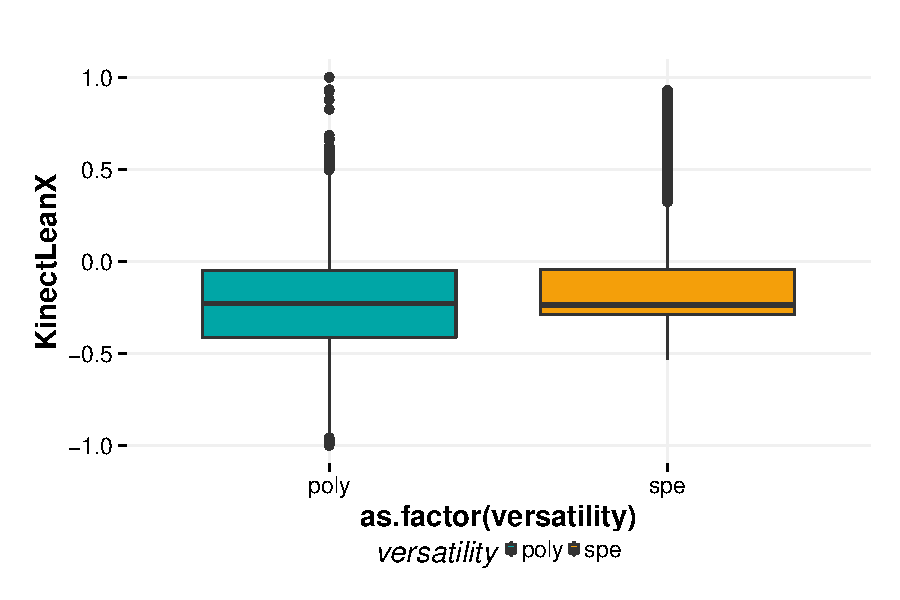
\includegraphics{features-plot_leanx_gender_quiz}

\begin{Schunk}
\begin{Soutput}
                        Df Sum Sq Mean Sq F value Pr(>F)    
factor(versatility)      1    258  258.37    3620 <2e-16 ***
Residuals           153721  10972    0.07                   
---
Signif. codes:  0 ‘***’ 0.001 ‘**’ 0.01 ‘*’ 0.05 ‘.’ 0.1 ‘ ’ 1
\end{Soutput}
\end{Schunk}


\textbf{Session}
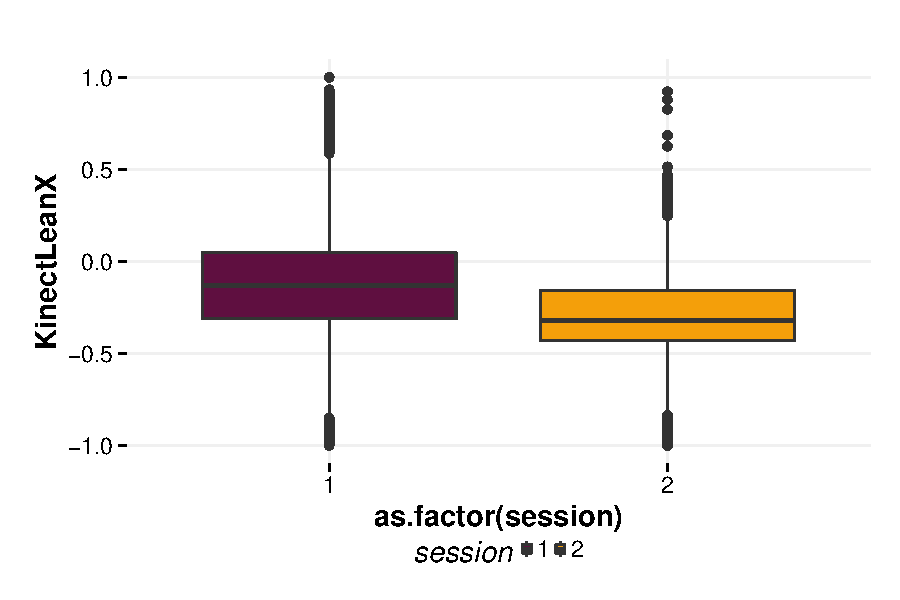
\includegraphics{features-plot_leanx_session_quiz}

\begin{Schunk}
\begin{Soutput}
Error: child
                Df Sum Sq Mean Sq F value Pr(>F)
factor(session)  1  166.6   166.6   0.727  0.416
Residuals        9 2061.7   229.1               

Error: Within
                    Df Sum Sq Mean Sq F value Pr(>F)    
factor(session)      1   1146  1145.9   22420 <2e-16 ***
Residuals       153711   7856     0.1                   
---
Signif. codes:  0 ‘***’ 0.001 ‘**’ 0.01 ‘*’ 0.05 ‘.’ 0.1 ‘ ’ 1
\end{Soutput}
\end{Schunk}

\textbf{Style}
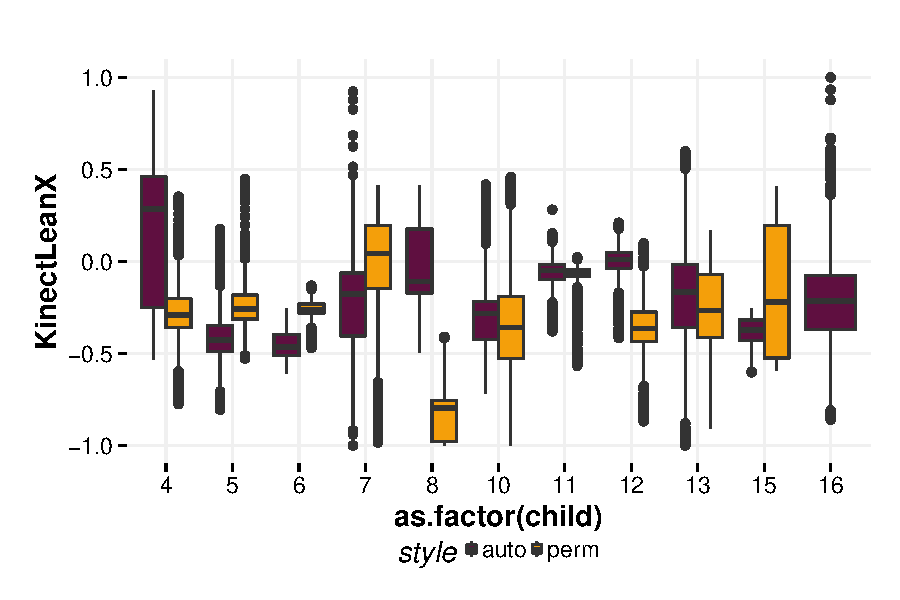
\includegraphics{features-plot_leanx_child_style_quiz}

\includegraphics{features-plot_leanx_style_quiz}

\begin{Schunk}
\begin{Soutput}
Error: child
              Df Sum Sq Mean Sq F value Pr(>F)
factor(style)  1   64.1   64.12     0.4  0.543
Residuals      9 1441.0  160.11               

Error: Within
                  Df Sum Sq Mean Sq F value Pr(>F)    
factor(style)      1   52.5   52.47    4909 <2e-16 ***
Residuals     153711 1642.9    0.01                   
---
Signif. codes:  0 ‘***’ 0.001 ‘**’ 0.01 ‘*’ 0.05 ‘.’ 0.1 ‘ ’ 1
\end{Soutput}
\end{Schunk}



\subsubsection{Hands Status}

\subsection{Dynamic Features}


\section{Postures}
% Table created by stargazer v.5.2 by Marek Hlavac, Harvard University. E-mail: hlavac at fas.harvard.edu
% Date and time: ven, oct 07, 2016 - 17:39:35
\begin{table}[!htbp] \centering 
  \caption{Summary statistics of activities metadata} 
  \label{} 
\begin{tabular}{@{\extracolsep{5pt}}lccccc} 
\\[-1.8ex]\hline 
\hline \\[-1.8ex] 
Statistic & \multicolumn{1}{c}{N} & \multicolumn{1}{c}{Mean} & \multicolumn{1}{c}{St. Dev.} & \multicolumn{1}{c}{Min} & \multicolumn{1}{c}{Max} \\ 
\hline \\[-1.8ex] 
ordre & 16 & 8.500 & 4.761 & 1 & 16 \\ 
age & 16 & 8.688 & 1.014 & 7 & 11 \\ 
p\_robot & 16 & 3.125 & 1.258 & 1 & 5 \\ 
p\_videogame & 16 & 3.500 & 1.414 & 1 & 5 \\ 
p\_bike & 16 & 2.375 & 1.310 & 1 & 5 \\ 
p\_book & 16 & 2.312 & 1.138 & 1 & 4 \\ 
p\_clothes & 16 & 3.688 & 1.537 & 1 & 5 \\ 
p\_homeworks & 16 & 3.375 & 1.147 & 1 & 4 \\ 
p\_play & 16 & 3.562 & 0.892 & 1 & 4 \\ 
p\_teach & 16 & 3.938 & 0.250 & 3 & 4 \\ 
p\_phone & 15 & 1.867 & 1.302 & 1 & 4 \\ 
p\_webbrowser & 15 & 2.067 & 1.335 & 1 & 4 \\ 
prefered\_session & 14 & 1.643 & 0.497 & 1 & 2 \\ 
e\_robot & 13 & 1.077 & 0.277 & 1 & 2 \\ 
e\_videogame & 13 & 2.615 & 1.193 & 1 & 5 \\ 
e\_bike & 12 & 3.250 & 0.965 & 2 & 5 \\ 
e\_book & 12 & 3.417 & 1.379 & 1 & 5 \\ 
e\_clothes & 13 & 4.308 & 0.751 & 3 & 5 \\ 
e\_homeworks & 13 & 3.115 & 0.650 & 2.000 & 4.000 \\ 
e\_play & 13 & 3.115 & 0.618 & 2.000 & 4.000 \\ 
e\_rules & 12 & 3.167 & 0.577 & 2 & 4 \\ 
e\_learn & 13 & 3.500 & 0.577 & 2.500 & 4.000 \\ 
e\_sport & 12 & 3.000 & 0.603 & 2 & 4 \\ 
e\_teach & 12 & 3.500 & 0.674 & 2 & 4 \\ 
e\_outside & 12 & 2.917 & 0.900 & 1 & 4 \\ 
e\_mood & 12 & 3.375 & 0.569 & 2.500 & 4.000 \\ 
e\_phone & 13 & 2.308 & 1.109 & 1 & 4 \\ 
e\_webbrowser & 13 & 2.500 & 0.957 & 1.000 & 4.000 \\ 
\hline \\[-1.8ex] 
\end{tabular} 
\end{table} 


\end{document}
